\documentclass{book}
\usepackage{graphicx}
\usepackage[english]{babel}
\usepackage{amsthm}
\usepackage{amssymb}
\usepackage{amsfonts}
\usepackage{mdframed}[framemethod=PSTricks]
\usepackage{physics}
\usepackage{tikz}
\usepackage[a4paper, margin=1in]{geometry}
\geometry{a4paper, margin=1in}
\usepackage{xcolor}
\usetikzlibrary{arrows.meta}
\usetikzlibrary{angles,quotes}
\graphicspath{ {./images/} }
\usepackage{svg}
\usepackage{subcaption}
\usepackage{bm}
\usepackage{empheq}
\usetikzlibrary{decorations.text}
\usepackage[most]{tcolorbox}
\usepackage{tensor}
\usepackage{cancel}
\usepackage{tcolorbox}
%3D
\usepackage{mathtools}
\usepackage{booktabs}
\usepackage{array}
\newcolumntype{C}{>{$}c<{$}}
\usepackage{tikz-3dplot}
\usepackage{appendix}
\usepackage{pgfplots}
\usetikzlibrary{shapes.geometric}
\usetikzlibrary{calc,patterns,angles,quotes}
%Tikz Library
\usetikzlibrary{angles, quotes, intersections}
\usepackage[bb=dsserif]{mathalpha}
\usetikzlibrary{decorations.pathmorphing}
\usepackage{tkz-euclide}
\tikzset{snake it/.style={decorate, decoration=snake}}

\usepackage{etoolbox} % ifthen
\usepackage[outline]{contour} % glow around text
\usetikzlibrary{calc} % for adding up coordinates
\usetikzlibrary{decorations.markings,decorations.pathmorphing}
\usetikzlibrary{angles,quotes} % for pic (angle labels)
\usetikzlibrary{arrows.meta} % for arrow size
\usepackage{xfp} % higher precision (16 digits?)
\tikzset{>=latex}
\usepackage{siunitx}
\usepackage{xcolor}
\colorlet{mygreen}{green!60!black}
\colorlet{myblue}{blue!70!black}
\colorlet{myred}{red!70!black}
\tikzstyle{rline}=[myred,thick]
\tikzstyle{bline}=[myblue,thick]
\tikzstyle{gline}=[mygreen,thick]
\pgfplotsset{compat=1.13} % TikZ coordinates <-> axes coordinates
%\pgfplotsset{compat=1.17}
\colorlet{mydarkblue}{blue!30!black}
\def\N{50}

% H2:  4u/2k =  4*1.66*10^(-27)/(2*1.38*10^(-23)) = 0.00024
% O2: 32u/2k = 32*1.66*10^(-27)/(2*1.38*10^(-23)) = 0.00192
% 4/sqrt(pi)
%\def\k{0.00024}
\pgfmathdeclarefunction{maxwell}{2}{%
	\pgfmathparse{4/sqrt(pi)*(\k/#2)^(3/2)*(#1^2)*exp(-\k*(#1^2)/#2)}%
}
\def\maxwell#1#2{4/sqrt(pi)*(\k/#2)^(3/2)*((\xscale*#1)^2)*exp(-((\xscale*#1)^2)*(\k/#2))}
%\def\vmax#1{sqrt(#1/\k)/\xscale}
\def\tick#1#2{\draw[thick] (#1) ++ (#2:0.03*\ymax) --++ (#2-180:0.06*\ymax)}



\renewcommand{\cleardoublepage}{\clearpage}

\title{Properties of Matter}
\author{Dominik Szablonski}
\newtheorem{law}{Law}
\newtheorem{klaw}{Law}
\newtheorem*{definition}{Definition}
\newtheorem*{theorem}{Theorem}
\newcommand{\dbar}{\mathrm{d}\hspace*{-0.08em}\bar{}\hspace*{0.1em}}
\pgfplotsset{compat=1.18}
\usepackage{graphicx}
\graphicspath{{./images/}}

\tikzstyle{atom}=[ball color=blue!50!black]
\tikzstyle{bound}=[thick,black!80,decorate,decoration={coil,amplitude=6pt,segment length=5pt}]


\begin{document}
	\global\mdfdefinestyle{blehgh}{%
		linecolor=black,middlelinewidth=2pt,%
		leftmargin=1cm,rightmargin=1cm
	}
	\mdfsetup{skipabove=\topskip,skipbelow=\topskip}
\maketitle

\tableofcontents

\chapter{Properties of Solids and Liquids}
\section{Introduction}
The kinetic energy per particle is $\approx k_BT$. Solids form when,
\begin{equation}
	k_BT << \epsilon
\end{equation}
where $\epsilon$ is the binding energy. Further, liquids form when,
\begin{equation}
	k_BT \approx \epsilon
\end{equation}
and gasses when,
\begin{equation}
	k_BT >> \epsilon.
\end{equation}
\section{Elasticity of Solids}
Solids exibit elastic behaviour, i.e., whenn stress is applied they deform (strain) and return to their original shape once removed. The way solids resist strain is defined by elastic moduli, which are general defined,
\begin{equation}
	\text{Elastic Modulus} = \frac{\text{Stress}}{\text{Strain}}.
\end{equation}
\subsection{Young's Modulus}
\begin{figure}
	\centering
	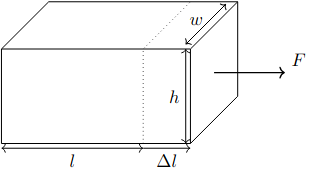
\includegraphics[width=175px]{Young'sModulus.png}
	\caption{Solid underegoing deformation due to a force along its axis.} \label{fig:young'smodulus}
\end{figure}
\begin{definition}
	$E$ - The ability of a solid to resist forces along a given axis.
\end{definition}\noindent
Consider a setup like in fig. \ref{fig:young'smodulus}. Stress is given by,
$
	\frac{F}{A}
$
and strain by,
$
	\frac{\Delta l}{l}
$
where $\Delta l$ is the deformation along the axis of the force. We then have,
\begin{equation}
	\boxed{E = \frac{F}{A}\left(\frac{\Delta l}{l}\right)^{-1}.}
\end{equation}
\subsection{Shear Modulus}
\begin{figure}
	\centering
	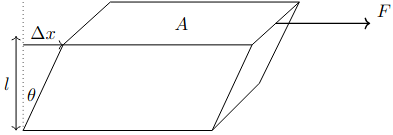
\includegraphics[width=200px]{shearmodulus.png}
	\caption{A solid undergoing shearing due to a force parallel to and along one of its faces.} \label{fig:shearmodulus}
\end{figure}
\begin{definition}
	$G$ - The ability of a solid to resist shearing when a force is applied parallel to the surface of the solid.
\end{definition}\noindent
Consider a setup like in fig. \ref{fig:shearmodulus}. If the solid shears by $\Delta x$ due to a force $F$, then its strain is,
\begin{equation}
	\frac{\Delta x}{l} = \tan\theta \approxeq \theta
\end{equation}
for small $\theta$. The shear modulus is then,
\begin{equation}
	\boxed{G = \frac{F}{A}\left(\frac{\Delta x}{l}\right)^{-1} = \frac{F}{A\theta}}.
\end{equation}
\subsection{Bulk Modulus}
\begin{figure}
	\centering
	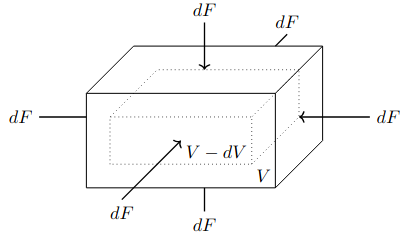
\includegraphics[width=220px]{bulkmodulus.png}
	\caption{A solid of volume $V$ being compressed by a force, $\dd{F}$, leading to an infinitesimal change in its volume $\dd{V}$.} \label{fig:bulkmodulus}
\end{figure}
\begin{definition}
	$K$ - Resistance of a material to compression.
\end{definition}\noindent
The bulk modulus describes the stress due to a change in pressure $\dd{P}$. If we consider a setup like in fig. \ref{fig:bulkmodulus}, the change in volume is $-\dd{V}$, the strain is $\dd{V}/V$, so the bulk modulus is,
\begin{equation}
	\boxed{K = -V \dv{P}{V}}.
\end{equation}
The minus sign indicates that an increase in pressure results in a decrease in volume.
\section{Properties of Static Liquids}
\subsection{Hydrostatic Pressure}
\begin{figure}
	\centering
	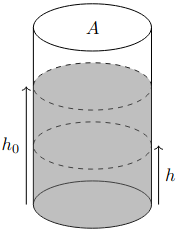
\includegraphics[height=150px]{hydrostatic.png}
	\caption{A column of liquid of constant density $\rho$, vertical height $h_0$, and cross-sectional area $A$.} \label{fig:hydrostatic}
\end{figure}
Consider a column of liquid of constant density $\rho_l$, a depth $d$, and cross-sectional area $A$ as in fig. \ref{fig:hydrostatic}. Since the liquid is static (no net flow), we have $F_{\text{net}} = 0$. The force at $d$ is then,
\begin{equation}
	F = P_0A + \rho d g A = P(d)Am
\end{equation}
so the pressure at $d$ is,
\begin{equation}
	\boxed{P(d) = P_0 + \rho g d}.
\end{equation}
$\implies$ as $d$ increases linearly, so does $P$.
\subsection{Buoyency and Archimedes Principle}
\begin{figure}
	\centering
	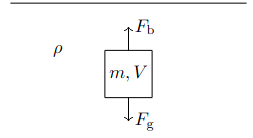
\includegraphics[width=150px]{archimedes.png}
	\caption{An arbitrary hollow shape of volume $V$ filled with liquid of density $\rho$, immersed in a liquid of the same density.} \label{fig:archimedes}
\end{figure}
Consider an arbitrary hollow shape of volume $V$ filled with liquid of density $\rho_l$, immersed in a liquid of the same density, as in fig. \ref{fig:archimedes}. The weight of the object is given by,
\begin{equation}
	F_w = \rho_l V g.
\end{equation}
The pressure acting on the body must be equal and opposite to its weight. We call this the \textit{buoyency force},
\begin{equation}
	\boxed{F_b = \rho_l V g}. \label{eq:buoyency}
\end{equation}
The buoyency force is \textit{equal and opposite to the weight of the liquid displaced}. I.e., in the case that the mass has a density $\rho_b$ such that $\rho_l > \rho_b$, the force it feels is still of the form eq. \eqref{eq:buoyency}, so will float above the surface of the water.
\section{Flow of Incompressible Liquid}
The molecules in a liquid or gas can easily flow, with the same time and position dependent velocity, $\vb{v}(\vb{r},t)$.
\subsection{Conservation of mass and the continuity equation}
The rate of mass flow through an area element of a surface $\dd{\vb{S}}$ is $\rho\vb{v}\cdot\dd{\vb{S}}$. The rate of mass flow into a volume bounded by a surface $S$ is this expression evaluated over all space,
\begin{equation}
	\dv{m}{t} = \rho\int_S\vb{v}\cdot\dd{\vb{S}}. \label{eq:RMF}
\end{equation}
For a liquid of constant density, eq. \eqref{eq:RMF} must equal $0$,
\begin{equation}
	\int_S \vb{v}\cdot\dd{\vb{S}} = 0
\end{equation}
and by the divergence theorem,
\begin{equation}
	\boxed{\div{\vb{v}} = 0}
\end{equation}
In the case of compressible liquids (i.e., where $\rho = \rho(\vb{r})$), conservation of mass is satisfied via the continuity equation,
\begin{equation}
	\boxed{\pdv{\rho}{t} + \div{(\rho\vb{v})} = 0}.
\end{equation}
\subsection{Bernoulli's Principle}
\begin{figure}
	\centering
	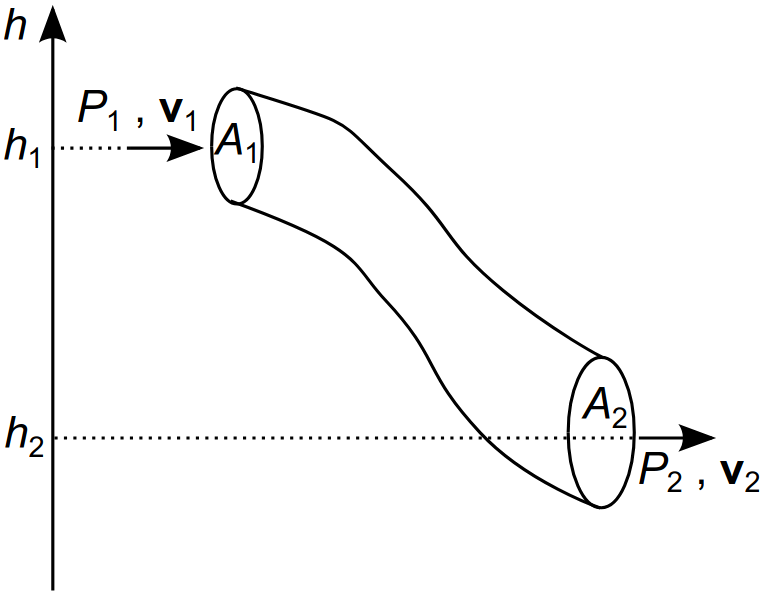
\includegraphics[width=200px]{bernouli.png}
	\caption{Frictionless pipe of arbitrary shape, with each end at a diffferent height $h_1$ and $h_2$ such that $h_2 < h_1$.} \label{fig:bernoulli}
\end{figure}
We will investigate how pressure of a liquid depends on flow speed. We assume no surface or iscous forces, and we assume flow is time independent, i.e., $\vb{v} = \vb{v}(\vb{r})$.\\\\
Particles will flow in streamlines. Consider adjacent streamlines which form a tube of arbitrary shape, where each end is at a different vertical height, $h_1$ and $h_2$ such that $h_2 < h_1$, and there is no flow in or out of the tube, as in fig. \ref{fig:bernoulli}. The liquid enters at height $h_1$, with velocity $v_1$, pressure $P_1$, through an area $A_1$. The liquid leaves at height $h_1$, with velocity $h_2$, pressure $P_2$, through an area $A_2$.
\\\\
From the conservation of mass,
\begin{equation}
	v_1A_1 = v_2A_2. \label{eq:consofmass}
\end{equation}
In a time $\dd{t}$, the work done by pressure $P_1$ on the liquid at entry is,
\begin{equation}
	\dd{W}_1 = P_1A_1v_1\dd{t}
\end{equation}
and similarly for the exit,
\begin{equation}
	\dd{W}_2 = P_2A_2v_2\dd{t}.
\end{equation}
The kinetic energy of the liquid is,
\begin{equation}
	\dd{K}_1 = \frac{1}{2}\left(\rho v_1A_1 \dd{t}\right)v_1^2,
\end{equation}
and the potential energy,
\begin{equation}
	\dd{V} = \left(\rho v_1A_1\dd{t}\right)gh_1,
\end{equation}
and similarly for the exit. By conservation of energy,
\begin{equation}
	\begin{split}
		\dd{W}_1 + \dd{K}_1 + \dd{V}_1 & = \dd{W}_2 + \dd{K}_2 + \dd{V}_2 \\
		A_1v_1\left(P_1 + \frac{1}{2}\rho v_1^2 + \rho g h_1\right)\dd{t} & = A_2v_2\left(P_2 + \frac{1}{2}\rho v_2^2 + \rho g h_2\right)\dd{t}
	\end{split}.\label{eq:conenergy}
\end{equation}
By eq. \eqref{eq:consofmass}, we can divide eq. \eqref{eq:conenergy} by $A_1v_1\dd{t}$,
\begin{equation}
	P_1 + \frac{1}{2}\rho v_1^2 + \rho g h_1 = P_2 + \frac{1}{2}\rho v_2^2 + \rho g h_2
\end{equation}
which leads to Bernoulli's equation,
\begin{equation}
	\boxed{P(h,v) + \rho g h + \frac{1}{2}\rho v^2 = \text{constant}}
\end{equation}
$\implies$ \textit{faster moving liquids have lower pressure}.
\subsection{Flow Properties and Viscocity}
\subsubsection{Laminar Flow}
\begin{definition}
	Smooth, regular streamlines that are locally parallel to each other
\end{definition}\noindent
The drag force on a spherical object of radius $R$ insterted into a liquid under laminar flow is caused by the liquid's resistance to shearing, and is given by Stoke's law,
\begin{equation}
	\boxed{\vb{F}_D = 6\pi \nu R\vb{v}}
\end{equation}
where $\nu$ is the viscocity of the liquid.
\subsubsection{Turbulent Flow}
\begin{definition}
	Streamlines are irregular and chaotic du to formation of eddies in the flow.
\end{definition}\noindent
The drag force on an object placed in the stream ocurs due to the inertial force required to push the liquid out of the way of the object. The drag force is given by,
\begin{equation}
	\boxed{\vb{F}_D = \frac{1}{2}\rho v^2 C_D A \vu{v}}
\end{equation}
where $A$ is the cross-sectional area of the object and $C_D$ is a dimensionaless drag coefficiant.
\subsubsection{Laminar-Turbulent Transition and Reynold's Number}
Whether a liquid expriences laminar or turbulent flow depends on the ratio of inertial force to viscous force. This ratio is given by Reynold's number,
\begin{equation}
	\boxed{Re = \frac{\rho L v}{\nu}}
\end{equation}
where $L$ is the length of the object moving through the liquid.
\section{Liquid Surfaces}
\textbf{Free Surface}: The surface interface of a liquid is characterised by the surface free energy $\gamma$. This is the energy required to increase the surface area of the interface.\\\\
\textbf{Liquid-Liquid Interface}: At the interface between two liquids, it is only energetically favourable for them to mix if $\gamma <0$.\\\\
\textbf{Liquid-Solid Interface}: For $\gamma < 0$, it is energetically favourable for the liquid to spread over the surface of the solid.
\subsection{Liquids in a Container}
\subsubsection{Contact Angle}
\begin{figure}
	\centering
	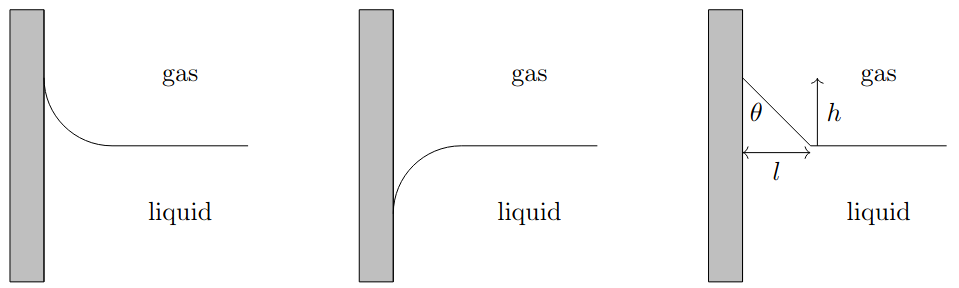
\includegraphics[width=400px]{contactangle.png}
	\caption{}\label{fig:contactangle}
\end{figure}
We are interested in the way a liquid-gas interface meets the solid wall of a container. The shape of the liquid near the wall is known as the meniscus, as in fig. \ref{fig:contactangle}. We can approximate the meniscus as linear, wehre the liquid meets the wall at the contact angle $\theta$, at a height $h$, and horizontal distance $l$ from the surface of the liquid.
\\\\
Let us consider the following surface-free energies,
\begin{enumerate}
	\item Solid-gas $\gamma_{sg}$,
	\item Solid-liquid $\gamma_{sl}$,
	\item Liquid-gas $\gamma_{lg}$.
\end{enumerate}
The meniscus free energy (per unit length of the meniscus, thus having dimensions of force) is given by,
\begin{equation}
	F_{\text{men}} = \left(\gamma_{sl} - \gamma_{sg}\right) + \gamma_{lg}\left(\sqrt{h^2 + l^2} - l\right).
\end{equation}
The free energy is minimised when,
\begin{equation}
	\pdv{F_{\text{men}}}{h} = \left(\gamma_{sl} - \gamma_{sg}\right) + \gamma_{lg}\left(\frac{1}{2}\frac{2h}{\sqrt{h^2 + l^2}}\right) = 0.
\end{equation}
We have that, 
\begin{equation}
	\frac{h}{\sqrt{h^2 + l^2}} = \cos\theta 
\end{equation}
which allows us to find Young's equation relating contact angle to surface free energy,
\begin{equation}
	\boxed{\gamma_{lg}\cos\theta = \gamma_{sg}-\gamma_{sl}}.
\end{equation}
\subsubsection{Capillary Action}
This occurs when a column of liquid is placed in a narrow tube. Consider a tube of radius $R$ at height $h$ relative to the surface of the bulk liquid. The surface free energy gain is,
\begin{equation}
	\Delta F_s = 2\pi r h \left(\gamma_{sl} - \gamma_{sg}\right)
\end{equation}
while the increase in gravitational potential energy is,
\begin{equation}
	\Delta F_g = \pi R^2 h \rho g \frac{h}{2}
\end{equation}
where $h/2$ is used as that is the location of the centre of mass.\\\\
The total free energy is,
\begin{equation}
	F = \Delta F_s + \Delta F_g = \frac{\pi}{2}R^2h^2\rho g + 2\pi Rh \left(\gamma_{sl} - \gamma_{sg}\right)
\end{equation}
which is minimised when,
\begin{equation}
	\pdv{F}{h} = \pi R^2 h \rho g + 2\pi R\left(\gamma_{sl} - \gamma_{sg}\right) = 0,
\end{equation}
which can be rearranged to give a function for $h$,
\begin{equation}
	\boxed{h = -\frac{2}{(\gamma_{sl} - \gamma_{sg})}{\rho g R} = \frac{2\gamma_{lg} \cos\theta}{\rho g R}}
\end{equation}
\subsection{Surface Tension and Surface Free Energy}
Consider a wire frame, with one side of length $l$, free to move in the $x$ direction. A thing iglm of liquid covers the space within the frame and shifts teh wire a distacen $\dd{x}$ in order ot minimise the overall free energy.\\\\
The work done on the wire to move a distance $\dd{x}$ due to a force $F$ applied by the thin film of liquid is,
\begin{equation}
	\dd{W} = F\dd{x}. \label{eq:workdone}
\end{equation}
The work also contributes to increasing the surface area of the liquid by,
\begin{equation}
	\dd{A} = sl \dd{x}.
\end{equation}
The energy increase is given by,
\begin{equation}
	\dd{E}_s = \gamma \dd{A} = 2\gamma l \dd{x}.\label{eq:energyincrease}
\end{equation}
Equating eq. \eqref{eq:workdone} and eq. \eqref{eq:energyincrease} gives an expression for the \textit{surface tension},
\begin{equation}
	\boxed{F = 2\gamma l}.
\end{equation}
\chapter{Thermodynamics}
In this chapter we deal with analysing the macroscopic properties of objects composed of many microscopic atoms and particles. We will first consider an idea gas, i.e., one in which,
\begin{itemize}
	\item the particles have no volume,
	\item and the particles have no interatomic forces acting between them.
\end{itemize}
This allows us to write down the ideal gas equation in two forms,
\begin{align}
	\boxed{\underbrace{P}_{\text{Pressure}}\overbrace{V}^{\text{Volume}} = \underbrace{n}_{\text{Moles}}\overbrace{R}^{\substack{\text{Molar gas }\\{\text{constant}}}}\underbrace{T}_{\text{Temperature}}} \\
	\boxed{PV = \underbrace{N}_{\substack{\text{Number of}\\\text{molecules}}} \overbrace{k_b}^{\substack{\text{Boltzmann}\\\text{constant}} } T}.
\end{align}
1 mole of substance contains $N_A$ (Avogadro's number) amount of molecules. We further have a relation between the molar gas constant and the Boltzman constant which states,
\begin{equation}
	R = N_Ak_b.
\end{equation}
In this course, we will often discuss 2 different variables,
\begin{enumerate}
	\item \textbf{Intensive Variables} - Value is not proportional to the amount of substance.
	\item \textbf{Extensive Variables} - Value is linearly proportional to the amount of substance. 
\end{enumerate}
\section{First law of thermodynamics}
\begin{law}
\begin{equation}
	\boxed{\underbrace{\Delta E}_{\substack{\text{Change in}\\\text{internal energy}} } = \underbrace{W}_{\substack{\text{Work done}\\\text{on the system}}} + \underbrace{Q}_{\substack{\text{Heat supplied}\\\text{to a system}}}}
\end{equation}
\end{law}
We say that $E$ is a function of state, meaning that the value of $E$ is path independent. For an ideal gas, we have that $E = E(T)$ which is the energy due to the kinetic energy of the particles. If we take the limit as $\Delta E \to 0$,
\begin{equation}
	\boxed{\dd{E} = \dbar Q + \dbar W}.
\end{equation}
Furthermore, $W$ and $Q$ are not functions of state, meaning that their values are path dependent. This means that,
\begin{equation}
	\Delta E = W + Q \equiv \text{Const}
\end{equation}
however, $W$ and $Q$ will not be constant as they depend on the shape of the function they take on.
\subsection{Cyclic Process}
This is a process which starts and ends in the same equilibrium state, so there is no change in energy over the cycle,
\begin{equation}
	\oint\dd{E} = E_{\text{final}} - E_{\text{initial}} = 0.
\end{equation}
From the first law,
\begin{equation}
	\oint \dbar{W} + \oint\dbar{Q} = 0
\end{equation}
and thus,
\begin{equation}
	\boxed{\oint\dbar{W} = -\oint \dbar{Q}}
\end{equation}
for a cyclic process.
\subsection{Quasistatic Process}
This is a process that occurs so slowly that the system is always instantaneously in thermal equilibrium. For a quasistatic process. the force applied is approximately equal to the pressure of the fluid itself,
\begin{equation}
	\boxed{\frac{\left|\vb{F}\right|}{A}\simeq P}.
\end{equation}
\subsection{Reversible Processes}
For a reversible process, we require,
\begin{enumerate}
	\item The process must be \textit{quasistatic}.
	\item There is no external friction.
	\item The process must not cause permanent change to the system.
\end{enumerate}
\subsubsection{Free expansion of an isolated gas}
\begin{figure}
	\centering
	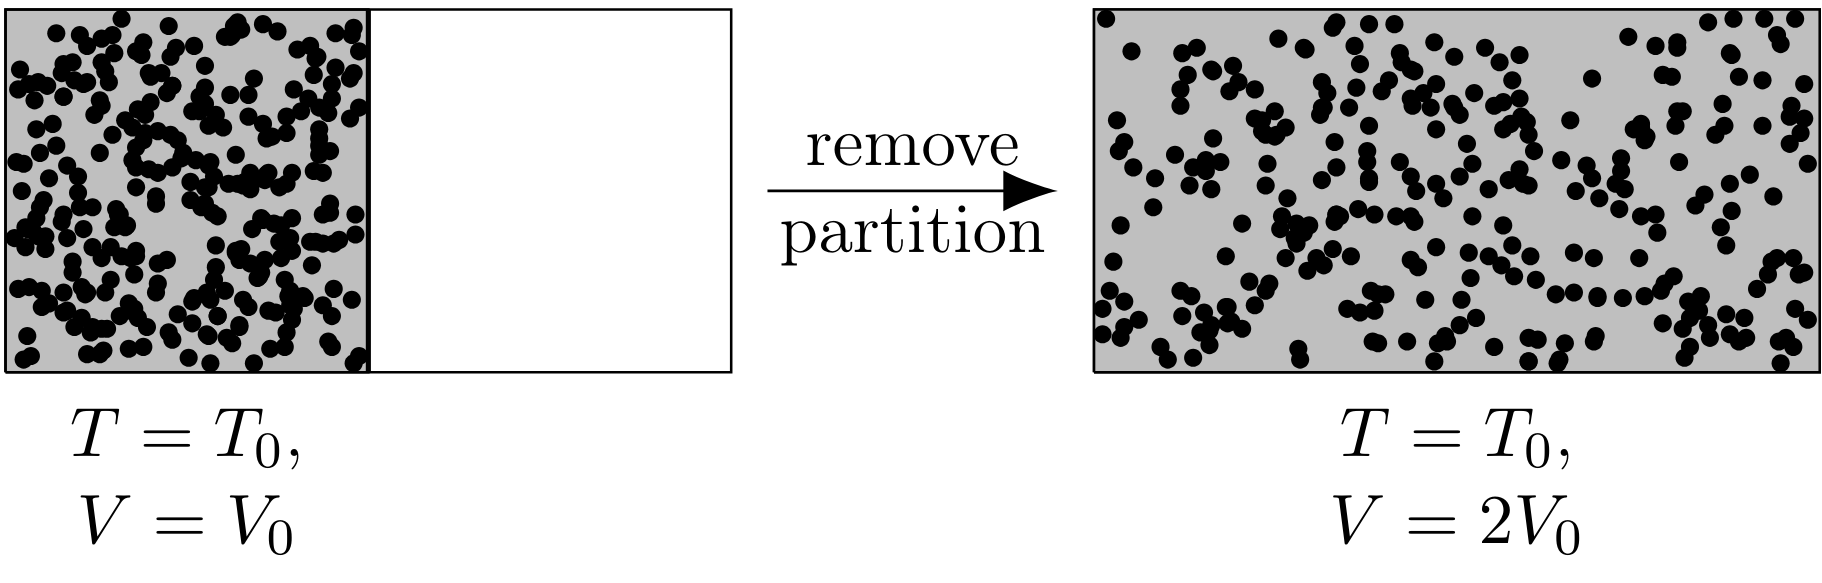
\includegraphics[width=300px]{FreeExpansion.png}
	\caption{} \label{fig:free expansion}
\end{figure}
Let us consider a gas confined in a volume which is seperated in half, with the gas initially in only one part of the volume as in fig. \ref{fig:free expansion}. If we remove the partition instantaneously, we have,
\begin{align}
	W = 0 && Q = 0 && \implies && \Delta E = 0.
\end{align}
However, this process is \textit{non-reversible}, as we have caused a permament change to the system.
\subsubsection{Isothermal expansion of an ideal gas}
\begin{figure}
	\centering
	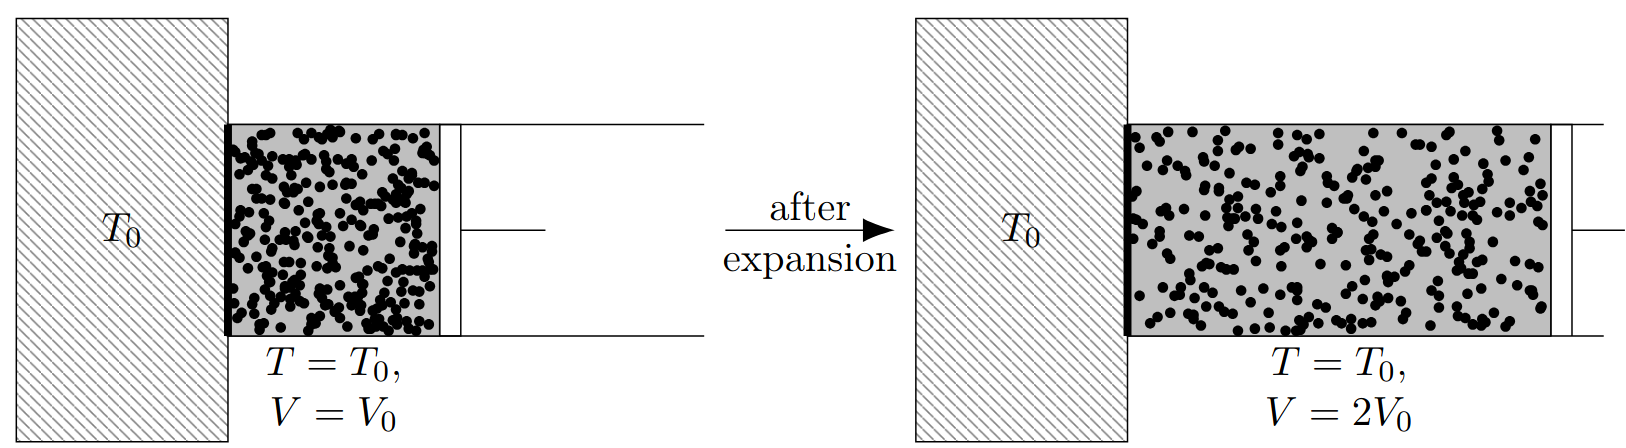
\includegraphics[width=300px]{Isothermal.png}
	\caption{} \label{fig:isothermal}
\end{figure}
Now consider a setup as in fig. \ref{fig:isothermal}, where we use a piston to change the volume of the container, and we use a source to keep the temperature of the gas constant. We have,
\begin{align}
	W < 0 && Q > 0 && \implies (Q+W) = 0 && \implies \Delta E = 0.
\end{align}
This process is \textit{reversible} given that,
\begin{itemize}
	\item The piston is frictionless,
	\item The piston moves slowly.
\end{itemize}
\subsection{Work Done}
Generally, the work done on a fluid is represented by an the area under the curve ono an \textit{indicator diagram}, which plots pressure against volume. If we consider a piston of cross-sectional area $A$ compressing a fluid, we can write the work done as,
\begin{equation}
	\boxed{\dbar W = \vb{F}\cdot\dd{\vb{x}} = \underbrace{\frac{|\vb{F}|}{A}}_P \underbrace{A\dd{x}}_{-\dd{V}} = -P\dd{V}}. \label{eq:work}
\end{equation}
For an ideal gas at temperature, we can evaluate this as,
\begin{equation}
	\begin{split}
	W & = -\int_{V_i}^{V_f} \frac{nRT}{V}\dd{V} \\
	& = nRT\ln\left(\frac{V_i}{V_f}\right).
	\end{split}
\end{equation}
For a cyclic process, the net work done is an enclosed area on the $P-V$ diagram.
\subsubsection{Reversible Work}
\begin{center}\textit{Stretching of a wire}\end{center}
If we have a string under tension $\Gamma$ which undergoes an infinitesimal change in length $\dd{\ell}$, we have,
\begin{equation}
	\dbar W = \Gamma \dd{\ell}.
\end{equation}
\begin{center}\textit{Increase in surface area}\end{center}
For a surface tension $\gamma$ and a change in area $\dd{A}$,
\begin{equation}
	\dbar W = \gamma \dd{A}.
\end{equation}
\subsection{Heat Capacity}
Heat capacity $C$ is the amount of energy required to raise the temperature by $\dd{T}$,
\begin{equation}
	\dbar Q = C\dd{T}.
\end{equation}
\subsubsection{Heat capacity at constant volume}
Rewriting the first law,
\begin{equation}
	\dbar Q = C_V\dd{T} = \dd{E} - \dbar W = \dd{E} + \underbrace{P\dd{V}}_0 \label{eq:9304}
\end{equation}
where the subscript $V$ indicates volume is being held constnat. We can take $P\dd{V}= 0$ since $V$ is constant, and $\Delta V \to 0, \dd{V} = 0$. Let us write $E = (V,T)$,
\begin{equation}
	\dd{E} = \pdv{E}{T}\dd{T} + \underbrace{\pdv{E}{T}\dd{V}}_0. \label{eq:2309}
\end{equation}
Equating eq. \eqref{eq:9304} to \eqref{eq:2309}, we get,
\begin{equation}
	\dbar{Q} = C_V\dd{T} = \pdv{E}{T}\dd{T}
\end{equation}
from which we obtain our final expression,
\begin{equation}
	C_V = \pdv{E}{T}.
\end{equation}
\subsubsection{Heat capacity at constant pressure}
Rewriting the first law,
\begin{equation}
	\dbar{Q} = C_P\dd{T} = \dd{E} + P\dd{V}.
\end{equation}
Writing $E = E(T, P)$,
\begin{equation}
	\dd{E} = \pdv{E}{T}\dd{T} + \underbrace{\pdv{E}{P}\dd{P}}_0.
\end{equation}
We can then obtain our final relation,
\begin{equation}
	\boxed{ C_P = \pdv{E}{T} + P\pdv{V}{T} }
\end{equation}
\subsubsection{Ideal Gas}
In an ideal gas, $E = E(T)$, i.e., energy has sole dependence on temperature. Thus,
\begin{equation}
	\dv{E}{T} = \pdv{E}{T} = C_V(T). \label{eq:20}
\end{equation}
From the ideal gas law,
\begin{equation}
	P\pdv{V}{T} = nR.
\end{equation}
From which we get the relation,
\begin{equation}
	\boxed{C_P(T) = C_V(T) + nR}.
\end{equation}
\subsection{Adiabatic Processes}
For an adiabtic procecss, there is \textit{no heat transfer}, i.e., $Q = 0$. From the first law and eq. \eqref{eq:20},
\begin{equation}
	\dd{E} - \dbar{W} = C_V\dd{T} - \dbar{W} = 0. \label{eq:203}
\end{equation}
From the ideal gas equation,
\begin{equation}
	T = \frac{PV}{nR}
\end{equation}
whose differential is,
\begin{equation}
	\dd{T} = \frac{1}{nR}\left(P\dd{V} + V \dd{P}\right)
\end{equation}
from which the differential of $E$ follows,
\begin{equation}
	\dd{E} = \frac{C_V}{nR}\left(P\dd{V} + V \dd{P}\right).\label{eq:020321}
\end{equation}
Substituting eq. \eqref{eq:020321} into eq. \eqref{eq:20} and assuming a reversible process ($\dbar W = - P \dd{V}$), we obtain,
\begin{equation}
	\begin{split}
		C_V \dd{T} + P\dd{V} = \frac{C_V}{nR}(P\dd{V}+V\dd{P}) + P \dd{V} & = 0 \\
		C_VV\dd{P} + \underbrace{(C_V nR)}_{C_P}P\dd{V} & = 0 \\
		\implies \frac{1}{P}\dd{P} + \frac{C_P}{C_V}\frac{1}{V}\dd{V} = 0. \label{eq:adiabtic}
	\end{split}
\end{equation}
If we have that $C_P$ and $C_V$ are constant, let us define,
\begin{equation}
	\gamma = \frac{C_P}{C_V}
\end{equation}
which is also constant. We can integrate eq. \eqref{eq:adiabtic} from $(P_1,V_1) \to (P_2, V_2)$,
\begin{equation}
	\begin{split}
	\int_{P_1}^{P_2}\frac{1}{P}\dd{P} + \gamma \int_{V_1}^{V_2}\frac{1}{V}\dd{V} & = 0
	\implies \ln\left(\frac{P_2V_2^{\gamma}}{P_1V_1^{\gamma}}\right) = 0 \label{eq:integrated}
	\end{split}
\end{equation}
Removing the logarithm from eq. \eqref{eq:integrated}, we obtain an expression relating the initial and final pressure and volume for an adiabatic process,
\begin{equation}
	\boxed{P_2V_2^{\gamma} = P_1V_2^{\gamma}}
\end{equation}
and by using the ideal gas law, we can eliminate variables and find expressions involving temperature,
\begin{align}
	\boxed{T_2V_2^{\gamma -1} = T_1V_1^{\gamma -1}} \\
	\boxed{T_2P_2^{\frac{1}{\gamma} - 1} = T_1P_1^{\frac{1}{\gamma} - 1}}
\end{align}
\section{Second Law of Thermodynamics}
\begin{law}
	The direction of heat flow approaches equillibrium, such that,
	\begin{itemize}
		\item Systems at an intermediate temperature reach equilibrium at an intermediate temperature.
		\item Heat naturally flows from hot bodies to cold bodies,
		\item We require an engine to produce work from heat.
	\end{itemize}
\end{law}
\subsection{Heat engines}

Heat engines produce work from heat. They operate in a cyclic process such that,
\begin{equation}
	\Delta E = \oint\dd{E} = 0.
\end{equation}
\subsubsection{Sterling Engine}
\begin{figure}
	\centering
	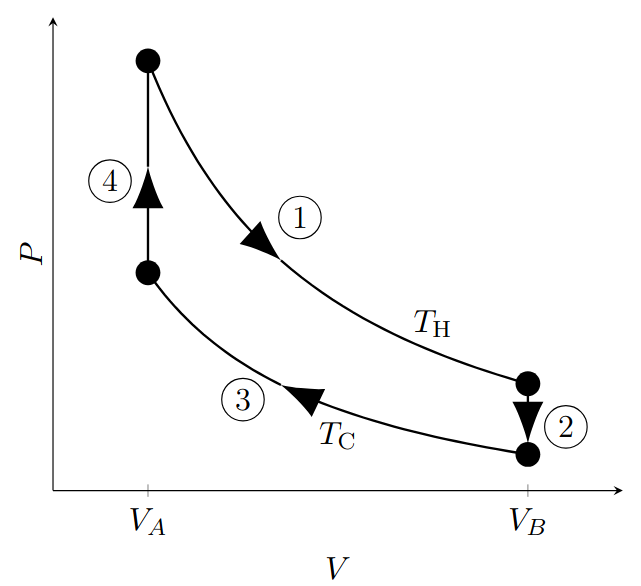
\includegraphics[width=200px]{heatengine.png}
	\caption{} \label{fig:heat engine}
\end{figure}
The Sterling engine is a piston operating between two heat reservoirs, with a hot reservoir at temperature $T_H$ and a hot reservoir at temperature $T_C$ where $T_C < T_H$ and contains an ideal gas. It works in a cycle such that,
\begin{enumerate}
	\item \textit{Isothermal expansion}
	\begin{itemize}
		\item Work done \textit{by} gas,
		\begin{equation}
			W_1 = nRT_H\ln{\left(\frac{V_B}{V_A}\right)}
		\end{equation}
		\item Heat \textit{absorbed},
		\begin{equation}
			Q_1 = W_1
		\end{equation}
	\end{itemize}
	\item \textit{Contact cooling}
	\begin{itemize}
		\item No work done.
		\item Heat \textit{ejected},
		\begin{equation}
			Q_2 = E(T_H) - E(T_C)
		\end{equation}
	\end{itemize}
	\item \textit{Isothermal compression}
	\begin{itemize}
		\item Work done \textit{on} gas,
		\begin{equation}
			W_3 = nRT_C\ln\left(\frac{V_B}{V_A}\right)
		\end{equation}
		\item Heat \textit{ejected}
		\begin{equation}
			Q_3 = W_3
		\end{equation}
	\end{itemize}
	\item \textit{Contact heating}
	\begin{itemize}
		\item No work done
		\item Heat \textit{absorbed},
		\begin{equation}
			Q_4 = E(T_H) - E(T_C)
		\end{equation}
	\end{itemize}
\end{enumerate}
This cycle can be visualised on an indicator diagram as in fig. \ref{fig:heat engine}. Furhthermore, this cycle can all be derived from the first law and $\dbar W = -P\dd{V}$. 
\\\\
Let us look at the cycle in more detail. The net work done \textit{by} the gas is,
\begin{equation}
	W = W_1 - W_3 = nR(T_H - T_C)\ln\left(\frac{V_B}{V_A}\right).
\end{equation}
The heat absorbed from the resevoir is at $T_H$ is,
\begin{equation}
	Q_H = Q_1 + Q_4.
\end{equation}
The heat ejected \textit{to} the hot resevoir is,
\begin{equation}
	Q_C = Q_2 + Q_3.
\end{equation}
From the first law,
\begin{equation}
	\Delta E = (-W) + (Q_H - Q_C) = 0
\end{equation}
and therefore,
\begin{equation}
	W = Q_H - Q_C = nR\ln\left(\frac{V_B}{V_A}\right)T_H + C_V\Delta T - nR\ln\left(\frac{V_B}{V_A}\right)T_C = nR\ln\left(\frac{V_B}{V_A}\right)\Delta T.
\end{equation}
where $\Delta T = T_H - T_C$. The efficiency of the engine is the ratio of desired output to required input, so,
\begin{equation}
	\eta_E = \frac{W}{Q_H}  = \frac{Q_H - Q_C}{Q_H} = \frac{nR\ln\left(\frac{V_B}{V_A}\right)\Delta T}{nR\ln\left(\frac{V_B}{V_A}\right)T_H + C_V\Delta T}.
\end{equation}
A schematic of the heat flow of a Sterling engine is shown in fig. \ref{fig:sterlingengine}.
\begin{figure}
	\centering
	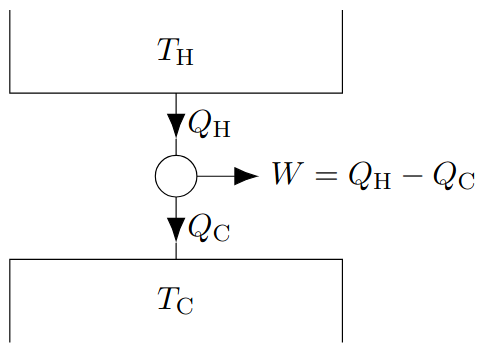
\includegraphics[width=150px]{sterlingengine.png}
	\caption{}\label{fig:sterlingengine}
\end{figure}
\subsection{Heat pumps and refrigirators}
These are the opposite of engines, they do work on a system to extract heat.
\subsubsection{Refrigerrator}
Work is done to extract heat $Q_C$ from a system to lower its temperature $T_C$. In this case, the efficiency of the system is given as,
\begin{equation}
	\eta_R = \frac{Q_C}{Q_H - Q_C}.
\end{equation}
\subsubsection{Heat Pump}
In a heat pump, we extract heat from a cooler resevoir at $T_C$ to heat a system to $T_H$. The desired ouput is $Q_H$, so,
\begin{equation}
	\eta_P = \frac{Q_H}{Q_H - Q_W}.
\end{equation}
If an engine is reversible, then,
\begin{equation}
	\eta_P = \frac{1}{\eta_E}.
\end{equation}
\subsection{Carnot's Cycle}

Carnot's theorem states,
\begin{theorem}
	\hspace{5px}
	\begin{enumerate}
		\item A reversible engine is most efficient.
		\item All reversible engines, operating between two heat baths, have the same efficiency, $\eta_C$ depending only on $T_H$ and $T_C$.
	\end{enumerate}
\end{theorem}\noindent
This type of engine can be constructed using the Carnot cycle (whose P-V diagram is shown in fig. \ref{fig:carnot}),
\begin{enumerate}
	\item \textbf{Isothermal Expansion} at $T_H$,
	\begin{itemize}
		\item $\Delta T = 0, \Delta E = 0$.
		\item $\dbar W = nRT_H\ln\left(\frac{V_B}{V_A}\right)$.
	\end{itemize}
	\item \textbf{Adiabatic Expansion}
	\begin{itemize}
		\item $\dbar Q \implies \dd{E} = \dbar W$
		\item $PV^{\gamma} = \text{Const.} \implies P \propto V^{-\gamma}$
		\item By the ideal gas law, $P = \frac{nRT}{V} \implies \frac{nRT}{V}V^{\gamma} = \text{Const.} \implies T_H V_B^{\gamma - 1} = T_CV_C^{\gamma -1}$.
	\end{itemize}
	\item \textbf{Isothermal Compression}
	\begin{itemize}
		\item $Q = nRT_C\ln\left(\frac{V_C}{V_D}\right)$
	\end{itemize}
	\item \textbf{Adiabatic Compression}
	\begin{itemize}
		\item $T_H V_A^{\gamma -1} = T_CV_D^{\gamma -1}$.
	\end{itemize}
\end{enumerate}
From the cycle above, we find that the ratio,
\begin{equation}
	\frac{V_B}{V_A} = \frac{V_C}{V_D}
\end{equation}
holds. From this, we can write down the efficiency of this engine,
\begin{equation}
	\eta_C  = \frac{W}{Q_H} = \frac{nRT_H\ln\left(\frac{V_B}{V_A}\right) - nRT_C\ln\left(\frac{V_C}{V_D}\right)}{nRT_H\ln\left(\frac{V_B}{V_A}\right)} = \frac{nRT_H\ln\left(\frac{V_B}{V_A}\right) - nRT_C\ln\left(\frac{V_B}{V_A}\right)}{nRT_H\ln\left(\frac{V_B}{V_A}\right)}
\end{equation}
from which we can write donw the final expression for the \textit{Carnot efficiency},
\begin{equation}
	\boxed{\eta_C = 1 - \frac{T_C}{T_H}}.
\end{equation}
Let us note that we find that the Stirling cycle approaches Carnot efficiency for small values of $C_V$.
\begin{figure}
	\centering
	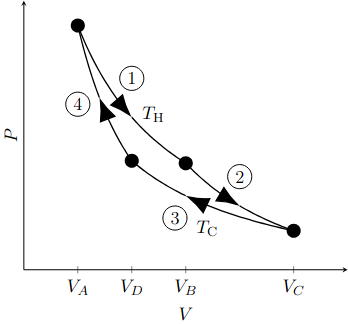
\includegraphics[width=150px]{carnot.png}
	\caption{} \label{fig:carnot}
\end{figure}
\subsection{Statements of the Second Law}
It is difficult to state the second law in a concise, general way through onyl understanding heat. However, below are two common formulations.

\subsubsection{Kelvin-Planck Statement}
\begin{tcolorbox}
	It is impossible to construct an engine which, operating in a cycle, produces no effect other than the extraction of heat from the reservoir and the performance of an equivalent amount of work.
\end{tcolorbox}

\subsubsection{Claussius Statement}
\begin{tcolorbox}
	It is impossible to construct a refrigirator which, operating in a cycle, produces no effect other than the transfer of heat from a cooler body to a hotter one.
\end{tcolorbox}
\section{Entropy}
Entropy is encoded into Calusiu's inequality, which states that if a system is taken over a cycle, absorbing infinitesimal amounts of heat $\dbar Q$, from various reservoirs at varing temperatures T, throughout, then
\begin{equation}
	\oint \frac{\dbar Q}{T} \leq 0.
\end{equation}
\subsection{Proof}
\begin{figure}
	\centering
	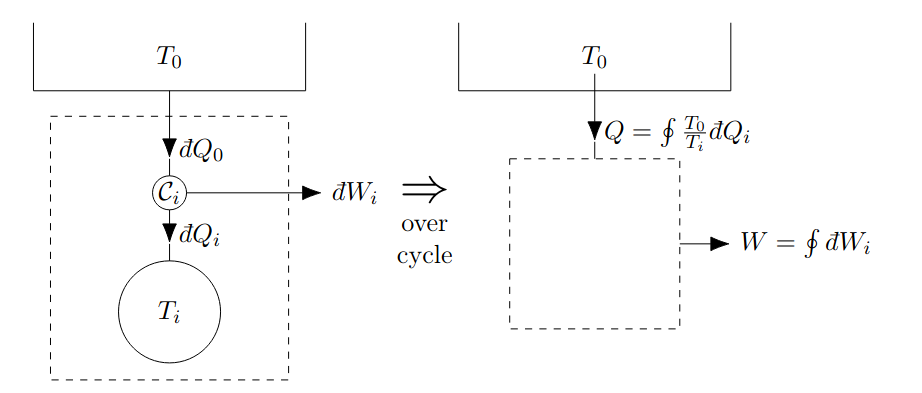
\includegraphics[width=0.7\textwidth]{clausius.png}
	\caption{}
	\label{fig:clausius}
\end{figure}
Let us consider a cycle as in fig. \ref{fig:clausius}. We have that the heat input is,
\begin{equation}
	Q_H = \oint\dbar Q_H = T_H \oint\frac{\dbar Q_i}{T_i}
\end{equation}
and the total work done is,
\begin{equation}
	W = \oint \dbar W_i.
\end{equation}
The only way for this cycle to be possible is if the work done is 0 or negative. Thus,
\begin{equation}
	\oint\dbar W_i \leq 0.
\end{equation}
We can write $\oint \dbar W_i = \oint \dbar Q_i$ and,
\begin{equation}
	\oint \frac{\dbar Q_i}{T_i} \leq 0.
\end{equation}
\subsection{Mathematical definition of entropy}
We define infinitesimal entropy of a system,
\begin{equation}
	\dd{S} = \frac{\dbar Q}{T}.
\end{equation}
\begin{figure}
	\centering
	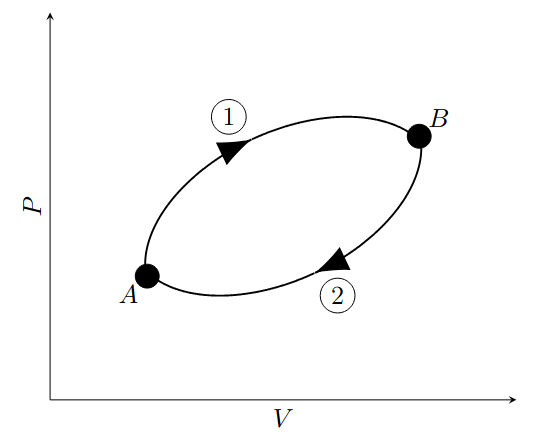
\includegraphics[width=0.5\textwidth]{cycle.png}
	\caption{}
	\label{fig:cycle}
\end{figure}
We only have constant entropy in equilibrium. Let us consider a process like in fig. \ref{fig:cycle}. The total entropy of this sytem is,
\begin{equation}
	\begin{split}
	&\oint\frac{\dbar Q}{T} = \int_A^B \frac{\dbar Q}{T} + \int_B^A \frac{\dbar Q}{T} = 0 \\
	\implies & \int_A^B \frac{\dbar Q}{T} - \int_A^B \frac{\dbar Q}{T} = 0
	\end{split}
\end{equation}
thus we have shown that entropy is path independent and thus is a function of state. Let us now define entropy further. Let us consider a reference state $O$ as we go from $A$ to $B$. We have,
\begin{equation}
	\begin{split}
		\int_A^B &= \int_A^O \frac{\dbar Q}{T} + \int_B^A \frac{\dbar Q}{T} \\
		& = \int_O^B \frac{\dbar Q}{T} - \int_O^A \frac{\dbar Q}{T}\\
		& = S(B) - S(A).
	\end{split}
\end{equation}
We can then define the entropy,
\begin{equation}
	\boxed{S(A) = \int_O^A \frac{\dbar Q_{\text{rev}}}{T}}.
\end{equation}
NOTE: Entropy is defined in terms of a reversible process.
\subsection{The law of increase in entropy}
Let us now consider a similar scenario to fig. \ref{fig:cycle}, but we have an irreversible process as we go from $A$ to $B$. Applying Clausius' inequality,
\begin{equation}
	\begin{split}
		\int_A^B \frac{\dbar Q_{\text{irrev}}}{T} + \int_B^A \frac{\dbar Q_{\text{rev}}}{T} & \leq 0\\
		\int_A^B\frac{\dbar Q_{\text{irrev}}}{T} \geq \int_A^B\frac{\dbar Q_{\text{rev}}}{T}
	\end{split}
\end{equation}
which gives us our final statement,
\begin{equation}
	S(B) - S(A) \geq \int_A^B \frac{\dbar Q_{\text{irrev}}}{T}
\end{equation}
\subsection{Thermally Isolated Systems}
For thermally isolated systems, it always holds that,
\begin{equation}
	S(B) - S(A) \geq 0.
\end{equation}
For a system doing the maximum amount of work, we have that,
\begin{equation}
	S(B) - S(A) = 0.
\end{equation}
For a system acting between two finite reservoirs, they will reach a final temperature given by,
\begin{equation}
	T_f = \sqrt{T_HT_C}.
\end{equation}
\subsection{Entropy and Heat Capacity}
Entropy can be used to define the heat capacity of for a given constant variable $X$. This is given by,
\begin{equation}
	C_X = T\left(\pdv{S}{T}\right)_X
\end{equation}
which, integrating, gives,
\begin{equation}
	S(T,X) - S(T_0, X) = \int_{T_0}^T \frac{C_X(T', X)}{T'}\dd{T'}.
\end{equation}
\subsection{Fundamental Relation of Thermodynamics}
The fundamental theorem of thermodynamics is a restatement of the second law,
\begin{equation}
	\boxed{\dd{E} = T\dd{S} + \dbar W_{\text{rev}}}.
\end{equation}
For an ideal gas, this is,
\begin{equation}
	\dd{E} = T \dd{S} - P\dd{V}.
\end{equation}
If we think of the second law, and energy being of the form $E \equiv E(S,V)$, we can write,
\begin{equation}
	\dd{E} = \left(\pdv{E}{S}\right)_V \dd{S} + \left(\pdv{E}{V}\right)_S \dd{V}
\end{equation}
which wen equating coefficients allows us to find,
\begin{align}
	\boxed{T = \left(\pdv{E}{S}\right)_V } && \boxed{P = -  \left(\pdv{E}{V}\right)_S}
\end{align}
\section{Thermodynamic Potentials}
From the fundamental relation of thermodynamics, we are able to derive different thermodynamic potentials, which allow us to state whether a reaction can happen spontaneously. 
\subsection{Work Availability}
We wish to find the maximum amount of work we can extract from a system initially out of equilibrium with the surroundings. A system like this will always increases its entropy if it can. We have that, for a system with the environment at pressure $P_0$ and temperature $T_0$, we have,
\begin{equation}
	\begin{split}
		\Delta S_{\text{tot}} & = \Delta S_{\text{sys}} + \Delta S_{\text{env}} \\
		& = \Delta S + \frac{Q}{T_0} \\
		& = \Delta S + \frac{-\Delta E - P\dd{V}}{T_0} \\
		& = \frac{T_0 \Delta S - \Delta E - P\dd{V}}{T_0} \geq 0
	\end{split}
\end{equation}
From this we can define the \textit{availability} of a system,
\begin{equation}
	- \Delta A = T_0 \Delta S - \Delta E - P\dd{V} \geq 0,
\end{equation}
for which we have that the entropy of a system increases given that $\Delta A \leq 0$. We can further interpret the availability as the useful work done by a system. We have that,
\begin{equation}
	\boxed{W_{\text{useful}} \leq -\Delta A}.
\end{equation}
We can further relate available work to thermodynamic potentials (described in detail in sections below).
\begin{itemize}
	\item For a process at constant temperature and pressure, the availability is related to the Gibbs free energy,
	\begin{equation}
		\boxed{W_{\text{usefull}} \leq -\Delta G}
	\end{equation}
	\item For a process at constant volume and temperature, the availability is related to the Helmholtz free energy,
	\begin{equation}
		\boxed{W_{\text{useful}} \leq -\Delta F}.
	\end{equation}
\end{itemize}
\subsection{Helmholtz Free Energy}
We can derive this from the Helmholtz free energy from the fundamental relation of thermodynamics,
\begin{equation}
	\begin{split}
		\dd{E} & = T\dd{S} - P\dd{V} \\
		& = T\dd{S} + S\dd{T} - S\dd{T} - P\dd{V} \\
		& = \dd{(TS)} - S\dd{T} - P\dd{V} \\
		\implies & \underbrace{\dd{E - TS}}_{\dd{F}} = \underbrace{- S \dd{T} - P \dd{V}}_{\dd{T} = 0, \dd{V} = 0}
	\end{split}
\end{equation}
From this we can define the Helmholtz free energy,
\begin{equation}
	\boxed{F(T,V) = E - TS}.
\end{equation}
Which holds for constnat $T$ and $V$. We can further consider the expansion of $\dd{F}$,
\begin{equation}
	\dd{F} = \left(\pdv{F}{T}\right)_V \dd{T} + \left(\pdv{F}{V}\right)_T \dd{V}
\end{equation}
and equating coefficients,
\begin{align}
	S = -\left(\pdv{F}{T}\right)_V && P = -\left(\pdv{F}{V}\right)_T.
\end{align}
We then have that,
\begin{equation}
	\dd{F} \leq 0
\end{equation}
where equality holds for equilibrium, and spontaneous change for $\dd{F} < 0$.
\subsection{Gibbs Free Energy}
We derive the Gibbs free energy from the Helmholtz free energy. We have,
\begin{equation}
	\begin{split}
		\dd{F} & = \dd{(E - TS)} = -S\dd{T} - P \dd{V} \\
		& = -S\dd{T} - p\dd{V} -v\dd{P} + V\dd{P} \\
		& = -S\dd{T} - \dd{(PV)} + V\dd{P} = \dd{(E - TS)} \\
		\implies & \underbrace{\dd{(E - TS + PV)}}_{\dd{G}} = -S\dd{T} + V\dd{P}
	\end{split}
\end{equation}
The Gibbs free energy is then,
\begin{equation}
	\boxed{G(T,P) = E - TS + PV}.
\end{equation}
The Gibbs free energy tells us about the non-reversible work in the system. Expanding $\dd{(E - TS + PV)}$, 
\begin{equation}
	\begin{split}
	& \dd{E} - \cancelto{0}{S\dd{T}} - T\dd{S} + P\dd{V} + \cancelto{0}{V\dd{P}} = \cancelto{0}{-S\dd{T}} + \cancelto{0}{V \dd{P}} \\
	\implies & \underbrace{\dd{E} - T\dd{S}}_{\dbar W_{\text{rev}}} + \underbrace{P\dd{V}}_{\dbar W_{\text{vol}}} = \dbar W_{\text{other}}
	\end{split}
\end{equation}
\subsection{Enthalpy}
Enthalpy is derived from the Gibbs free energy. We consider enthalpy at constant entropy and pressure. Furthermore, for a system at constant pressure, the enthalpy is interpreted as the heat released during the process. The derivation is shown below,
\begin{equation}
	\begin{split}
	\dd{(E - TS + PV)} & = -S \dd{T} + V\dd{P} \\
	& = -S\dd{T} -T\dd{S} + T\dd{S} + V\dd{P} \\
	& = - \dd{(TS)} + T\dd{S} + V\dd{P} \\
	\implies \dd{(E + PV)} & = T\dd{S} + V\dd{P}
	\end{split}
\end{equation}
we then define the enthalpy $H$,
\begin{equation}
	H = E + PV
\end{equation}
where we have,
\begin{equation}
	\boxed{\dd{H} = T\dd{S} V\dd{P}}
\end{equation}
and the relations,
\begin{align}
	\left(\pdv{H}{S}\right)_P = T && \left(\pdv{H}{P}\right)_S = V.
\end{align}
We can further define the Gibbs free energy in terms of enthalpy,
\begin{equation}
	\dd{G} = \dd{H} - T\dd{S}
\end{equation}
where we require $\dd{G} \leq 0$ for spontaneous change.
\subsection{Interpretation of Thermodynamic Potentials}
\subsubsection{Internal Energy}
For thermally isolated systems, ($Q = 0$),
\begin{equation}
	\begin{split}
	& \Delta A = \Delta E + P_0\Delta V = 0 \\
	\implies & \Delta E = - P_0 \Delta V.
	\end{split}
\end{equation}
\subsubsection{Entropy}
For thermally isolated systems at fixed volume,
\begin{equation}
	\Delta A = - T_0 \Delta S
\end{equation}
thus,
\begin{equation}
	(\Delta S)_{E,V} \geq 0
\end{equation}
for spontaneous change. I.e., entropy must be maximised.
\subsubsection{Helmholtz Free Energy}
For a system that starts and ends at the same temperature, with constant volume,
\begin{equation}
	\Delta A = \Delta (E - T_0 S) = \Delta F
\end{equation}
so,
\begin{equation}
	(\Delta F)_{T,V} \leq 0
\end{equation}
for spontaneous change.
\subsubsection{Gibbs Free Energy}
If the system starts and ends at the same pressure and temperature, the availability becomes,
\begin{equation}
	\Delta A = \Delta (E - T_0S + P_0V) = \Delta G
\end{equation}
thus for spontaneous change,
\begin{equation}
	(\Delta G)_{T,P} \leq 0
\end{equation}
and for equilibrium, we minimise the Gibbs free energy.
\subsubsection{Enthalpy}
For a system at constant pressure, the work done is $P_0\Delta V$. From the first law,
\begin{equation}
	\Delta E = Q - P_0 \Delta V.
\end{equation}
The change in enthalpy is,
\begin{equation}
	\Delta H = \Delta E + P_0 \Delta V
\end{equation}
and we therefore have,
\begin{equation}
	(\Delta H)_P = Q
\end{equation}
so the change in enthalpy is the heat released during a process.
\subsection{Maxwell Relations}
The Maxwell relations are given below, with proof given for the first below,
\begin{tcolorbox}
	\begin{align}
		\left(\pdv{P}{S}\right)_V &= - \left(\pdv{T}{V}\right)_S \label{eq:maxwell 1}\\
		\left(\pdv{S}{V}\right)_T &= \left(\pdv{P}{T}\right)_V \\
		\left(\pdv{T}{P}\right)_S &= \left(\pdv{V}{S}\right)_P \\
		\left(\pdv{S}{P}\right)_T &= - \left(\pdv{V}{T}\right)_P 
	\end{align}
\end{tcolorbox}\noindent
We will show the proof for eq. \eqref{eq:maxwell 1}, but the proofs for all other relations follow similarly.
\begin{proof}
	\begin{equation*}
		\begin{split}
			\dd{E} = T\dd{S} - P\dd{V} = \left(\pdv{E}{S}\right) \dd{S} + \left(\pdv{E}{V}\right)_S \dd{V}
		\end{split}
	\end{equation*}
	\begin{align*}
		T = (\pdv{E}{S})_V && P = -\left(\pdv{E}{V}\right)_S
	\end{align*}
	\begin{equation*}
		\begin{split}
			\pdv{V}\left(\pdv{E}{S}\right)  & = \pdv{S}\left(\pdv{E}{V}\right)\\
			\implies \left(\pdv{P}{S}\right)_V & = - \left(\pdv{T}{V}\right)_S 
		\end{split}
	\end{equation*}
\end{proof}
\section{Phase Transitions}
In order to consider phase transitions, we must consider \textit{open systems}, i.e., systems where the number of particles can change. We can then write the internal energy to account for open systems,
\begin{equation}
	E = TS - PV + \mu N
\end{equation}
where $\mu$ is the chemical potential. We can then write the FTR,
\begin{equation}
	\dd{E} = T\dd{S} - P\dd{V} + \mu \dd{N}.
\end{equation}
We can visualise phase transitions on a P-T diagram, as in figure \ref{fig:pt},
\begin{figure}
	\centering
	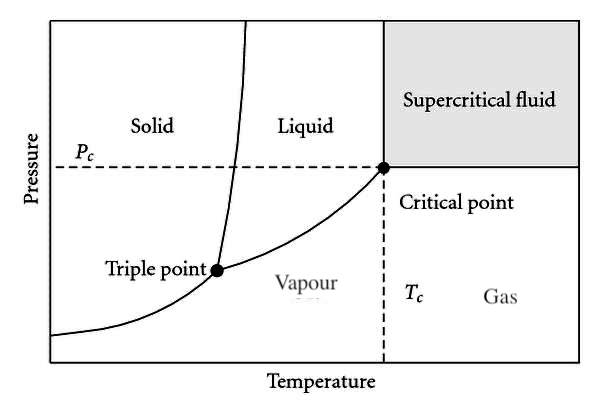
\includegraphics[width=0.5\textwidth]{P-T-diagram.png}
	\caption{}
	\label{fig:pt}
\end{figure}
\subsection{Phase Transition Conditions}
For a substance to transition from one state to another, it must be possible for the two states to be in equilibrium. Considering a total isolated systems composed of two systems in two different states,
\begin{equation}
	S(E,V,N) = S_1(E_1, V_1, N_1) + S_2(E_2,V_2,N_2)
\end{equation}
Considering $\dd{S}$ for each part of the system, we obtain the differentials,
\begin{align}
	\left(\pdv{S_1}{E_1}\right)_{V_1,N_1} = \left(\pdv{S_2}{E_2}\right)_{V_2,N_2} \\
	\left(\pdv{S_1}{V_1}\right)_{E_1,N_1} = \left(\pdv{S_2}{V_2}\right)_{E_2,N_2}\\
	\left(\pdv{S_1}{N_1}\right)_{E_1,V_1} = \left(\pdv{S_2}{N_2}\right)_{E_2,V_2}
\end{align}
These lead to the conditions for phase equilibrium,
\begin{tcolorbox}
	\begin{itemize}
		\item $T_1 = T_2$, no heat flow between systems.
		\item $P_1 = P_2$, the systems are at mechanical equilibrium.
		\item $\mu_1 = \mu_2$, there is no preference to be in one state over another.
	\end{itemize}
\end{tcolorbox}
\subsection{Clausius-Clapeyron Relation}
If we approximate the interface line between two states as being linear, such that we go from points $(T,P) \to (T+\delta T, P + \delta P)$, we can write the Clausius-Clapeyron relation as,
\begin{equation}
	\frac{\delta P}{\delta T} = \frac{\Delta H}{T \Delta\mathcal{V}}
\end{equation}
where $\mathcal{V}$ is the molar volume, and $\Delta H$ is the molar change in enthalpy, often written as $L$, and referred to as the latent heat.
\subsection{Liquid Gas-Transition}
\begin{figure}
	\centering
	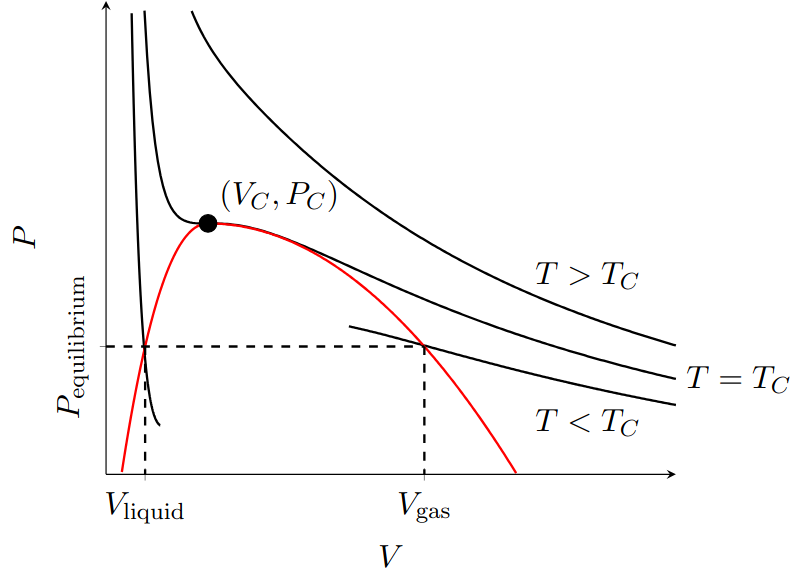
\includegraphics[width=0.6\textwidth]{pv phase.png}
	\caption{}
	\label{fig:pv phase}
\end{figure}
We wish to anallyse the liquid-gas transition more carefully. With the liquid-gas coexistance line ending at the critical point, we can infer that it is possible we can reach the gas phase from the liquid phase without a phase transitition. Thus, we could describe both liquid and gas with the same equation of state. If we insepct the $P-V$ diagram in figure \ref{fig:pv phase}, we see that at there is a saddle point at the critical point,
\begin{align}
	\left(\pdv{P}{V}\right)_{T_C} = 0 && \left(\pdv[2]{P}{V}\right)_{T_C} = 0 \label{eq:fkjhdsklaj}
\end{align}
Below the critical point, we see there is a region where we have unstable states, known as supercooled or superheated states.
\subsection{Real Gasses}
In order to describe the liquid phase, we must take into account interactions between molecules. This is encoded in the van der Walls equation,
\begin{equation}
	\boxed{\left(P + \frac{n^2a}{V^2}\right)\left(V - nb\right) = RT}.
\end{equation}
The Van der Walls equation reduces to the ideal gas equation when $V > nb$, where in turn $V >> \sqrt{a/P}$. If we apply eq. \eqref{eq:fkjhdsklaj} to the Van der Wall's equation, we obtain the critical values for a fluid at the critical point,
\begin{align}
	V_c = 3b, && T_C = \frac{8a}{27Rb}, && P_c = \frac{a}{27b^2}
\end{align}
If we analyse the isotherms produces by the Van der Wall's equation, as in figure \ref{fig:pv van}, we find that instability occurs due to positive gradients on the PV diagram.
\begin{figure}
	\centering
	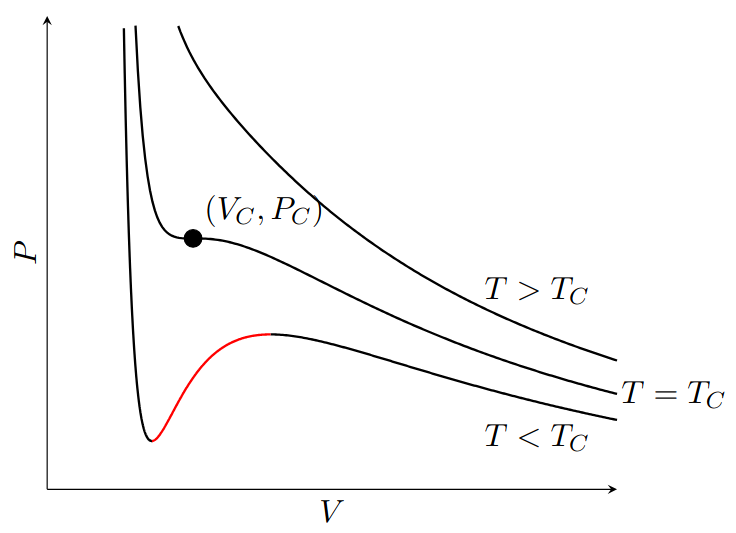
\includegraphics[width=0.5\textwidth]{pv van.png}
	\caption{}
	\label{fig:pv van}
\end{figure}
\chapter{Kinetic Theory of Gasses}
\section{Probability Distributions}
Given a probability distribution $p(\vb{v})$,
\begin{equation}
	P = \int p(\vb{v}) \dd^3v
\end{equation}
is the probablility of a particle having a velocity vector $\vb{v}$ between $\vb{v}$ and $\vb{v} + \dd^3v$, i.e., that the particle's velocity will be found in a box of dimensions $\dd{v}_x\dd{v}_y\dd{v}_z$. Below are listed some properties of probability distributions,
\begin{itemize}
	\item $p(\vb{v}) \geq 0$ $\forall \vb{v}$.
	\item The distribution is normalised, $\int_{-\infty}^{\infty} p(\vb{v})\dd^3v = 1$.
	\item For independent, uncorrelated variables,
	\begin{equation}
		p(\vb{v}) = p(v_x)p(v_y)p(v_z)
	\end{equation}
	\item The mean value of a quantity described by $f(\vb{v})$ is given by,
	\begin{equation}
		\left<f\right> = \int f(\vb{v})p(\vb{v})\dd^3v.
	\end{equation}
	\item The variance is given by,
	\begin{equation}
		\sigma^2(f) = \left<f^2\right> - \left<f\right>^2.
	\end{equation}
\end{itemize}
\subsection{Gaussian Integrals}
Guassian integrals of the $m^{\text{th}}$ order have the form,
\begin{equation}
	I_m = \int_{-\infty}^{\infty}x^{m}e^{-ax^2}\dd{x}
\end{equation}
for $a > 0$. We can relate even gaussian integrals by,
\begin{equation}
	I_{2n} = \dv[n]{a}I_0.
\end{equation}
\section{The Boltzmann Factor}
For a fixed number of paticles in thermall equilibrium at temperature $T$,
\begin{equation}
	\boxed{p(\text{state}) \propto \exp\left(-\frac{E(\text{state})}{k_BT}\right)}
\end{equation}
\begin{itemize}
	\item As $T \to \infty$, all states have equal probability
	\item As $T \to 9$, lowest energy states have higher probability.
\end{itemize}
If we wish to use this probability distribution, we must first normalise it, such that,
\begin{equation}
	p(\text{s}) = \frac{1}{Z}\exp\left(-\frac{E(\text{s})}{k_BT}\right)
\end{equation}
where the normalisation constant is,
\begin{equation}
	Z = \int_{\text{all states}}\exp\left(-\frac{E(\text{s})}{k_BT}\right)\dd{s}
\end{equation}
\subsection{Example: Isothermal Atmosphere}
If we consider a planet that has an atmosphere consisting of a gas of non-interacting molecules with mass $m$, temperature $T$, with an acceleration due to gravity $g$ at a height $y$ above the planet's surface, we can describe the probability of finding a particle at a height $y$ using teh Boltzmann factor. A single particle will be subject to a potential $mgy$, so its probability distribution will be,
\begin{equation}
	p(y) = \frac{1}{Z} \exp \left(-\frac{mgy}{k_BT}\right)
\end{equation}
which is normalised by,
\begin{equation}
	Z = \int_0^\infty \exp\left(-\frac{mgy}{k_BT}\right) \dd{y} = \frac{k_BT}{mg}.
\end{equation}
We understand that an atmosphere is made up of more than 1 molecule of gas. For non-interacting molecules, we can say that the density of the gas is proportional to its probability density, $\rho(y) \propto p(y)$, such that,
\begin{equation}
	\rho(y) = \rho_0 \exp \left(-\frac{mgy}{k_BT}\right).
\end{equation}
If we consider pressure due to the weight of the particles, for an incremental increase in height $\dd{y}$, the chanve in pressure is given by $\dd{P} = - \rho g \dd{y}$. We can then write,
\begin{equation}
	\begin{split}
		P(y) & = \int_{\infty}^{y}-\dd{P} = -g\rho_0 \int_{-\infty}^{y}\exp\left(-\frac{mgy}{k_BT}\right) \\
		& = \frac{k_BT}{m}\rho_0 \exp\left(-\frac{mgy}{k_BT}\right)  = \frac{k_BT}{m}\rho(y).
	\end{split}
\end{equation}
If we consider $\frac{\rho}{m} = \frac{N}{V}$ where $N$ is the number of molecules, we get
\begin{equation}
	PV = Nk_BT
\end{equation}
whcih is the ideal gas law.
\subsection{Equation of State of an Ideal Gas}
Let us find the equation of an ideal gas more generally using the velocity distribution of an ideal, homogenous, isotropic gas in a cubic container. Particles in a gas have velocities,
\begin{equation}
	\vb{v} = \left(\Dot{x}, \Dot{y}, \Dot{z}\right) 
\end{equation}
and kinetic energy,
\begin{equation}
	K = \frac{1}{2}mv^2 = \frac{1}{2}m\left(\Dot{x}^2 + \Dot{y}^2 + \Dot{z}^2\right).
\end{equation}
The velocity distribution is going to be given by $p(\vb{v}) = p(\Dot{x})p(\Dot{y})p(\Dot{z})$. Inserting $\Dot{x}$ into the Boltzmann distribution,
\begin{equation}
	p(\Dot{x}) = \frac{1}{Z} \exp\left(\frac{\frac{1}{2}m\Dot{x}^2}{k_BT}\right).
\end{equation}
Normalising this integral,
\begin{equation}
	\begin{split}
	Z &= \int_{-\infty}^{\infty}\exp\left(\frac{\frac{1}{2}m\Dot{x}^2}{k_BT}\right) \dd{x}
	\\ & = \left(\frac{2\pi K_bT}{m}\right)^{\frac{1}{2}}
	\end{split}
\end{equation}
which we evaluate by a standard solution to the $0^{\text{th}}$ order Gaussian integral. The probability distribution is then,
\begin{equation}
	p(\Dot{x}) = \left(\frac{m}{2\pi K_bT}\right)^{\frac{1}{2}} \exp\left(\frac{\frac{1}{2}m\Dot{x}^2}{k_BT}\right).
\end{equation}
Following similar steps for $\Dot{y}$ and $\Dot{z}$, the probability distribution is given by,
\begin{equation}
	p(\vb{v}) = \left(\frac{m}{2\pi K_bT}\right)^{\frac{1}{2}} \exp\left(\frac{\frac{1}{2}mv^2}{k_BT}\right).
\end{equation}
If we evaluate the average velocity for each component, we find that,
\begin{equation}
	\left<\Dot{x}\right> = \left<\Dot{y}\right> = \left<\Dot{z}\right> = 0
\end{equation}
which is expected, as given that the gas is homogeneous and isotropic, we expect the particles to move in all directions equally.
\subsubsection{Pressure in container}
\begin{figure}
	\centering
	\usetikzlibrary{3d}
	\begin{tikzpicture}
		\draw (0,0,0) -- (2,0,0) -- (2,0,2) -- (0,0,2) -- (0,0,0) -- (0,2,0) -- (0,2,2) -- (0,0,2);
		\draw (0,2,2) -- (2,2,2) -- (2,0,2) -- (2,0,0);
		\draw (2,2,2) -- (2,2,0) -- (0,2,0);
		\draw (2,2,0) -- (2,0,0);
		\draw[<->] (3, 0, 1) -- (3, 2, 1) node[anchor = west, midway] {$\dot{x} \dd{t}$};
		\draw[->] (-2, 0.5, 0) -- (-2, -1, 0) node[anchor=east, align=center] {$x$};
		\draw[->] (0.5,1,2) -- (1,0,1) node[midway, anchor = north east] {$\vb{v}$};
		\draw[->] (1,0,1) -- (1,1,0.5) node[midway, anchor = west] {$\vb{v}'$};
	\end{tikzpicture}
	\caption{Incoming particle undergoes an elastic collision with one surface of the box.}
	\label{fig:col}
\end{figure}
Consider an elastic collision with one surface of area $A$ of the box in a small time $\dd{t}$ as in figure \ref{fig:col}. The volume from which the particles collide is $\Dot{x}A\dd{t}$. Given the number density $n = N/V$, thte total number of particles coliding with the surface in a time $\dd{t}$ is,
\begin{equation}
	N_{\text{col}} = n\Dot{x}A \dd{t}.
\end{equation}
Each collision transfers $2m\Dot{x}$ of momentum to the sruface due to elastic collisions. The average momentum transfer in a time $\dd{t}$ is given by,
\begin{equation}
	\begin{split}
	\dd{\bar{p}_m} & = nA\dd{t}2m\left<\Dot{x}^2\right> \\
	& = 2mnA\dd{t} \int_0^{\infty} \Dot{x} ^2 p(\Dot{x})\dd{\Dot{x}}.
	\end{split}
\end{equation} 
The force on the surface is,
\begin{equation}
	F = \dv{\bar{p}_m}{t} = 2mnA \int_0^{\infty} \Dot{x} ^2 p(\Dot{x})\dd{\Dot{x}}.
\end{equation}
The total pressure is then,
\begin{equation}
	\begin{split}
		P = \frac{F}{A} & = 2mn\left(\frac{m}{2\pi K_bT}\right)^{\frac{1}{2}} \int_0^{\infty} \Dot{x}^2 \exp\left(\frac{\frac{1}{2}m\Dot{x}^2}{k_BT}\right) \dd{\Dot{x}} \\
		& = 2mn\left(\frac{m}{2\pi K_bT}\right)^{\frac{1}{2}} \frac{1}{4}\left(\frac{\pi(2k_BT)^3}{m^3}\right) \\
		& = nk_B T = \frac{N}{V}k_BT \implies \boxed{PV = Nk_B T}
	\end{split}
\end{equation}
and thus we have derived the ideal gas law from statistical considerations.
\subsection{Internal Energy of an Ideal Gas}
\begin{figure}
	\centering
	\begin{tikzpicture}
		\draw[->] (-2.5, 0) -- (2.5, 0) node[anchor=west] {$\Dot{x}$};
		\draw[->] (0,-2.5) -- (0,2.5) node[anchor = south] {$\Dot{y}$};
		\coordinate (O) at (0,0);
		\draw (O) circle (1.5);
		\draw (O) circle (1.7);
		\coordinate [label = left:$\vb{v}$] (v) at (45:1.5);
		\draw[->] (O) -- (v);
		\node at (v)[circle, fill, inner sep =1pt]{};
		\draw[<->] (25:1.5) -- (25:1.7) node[right] {$\dd{\vb{v}}$};
	\end{tikzpicture}
	\caption{Sphere in velocity space at $\Dot{z} = 0$.}
\end{figure}
In an ideal gas, the only energy that exists is kinetic energy. So, the mean energy is given by,
\begin{equation}
	\begin{split}
	\left<E\right> & = N \int \frac{1}{2}mv^2 p(\vb{v}) \dd^3 v \\
	& = \frac{1}{2}Nm\left(\frac{m}{2\pi k_BT}\right)\int v^2 \exp\left(-\frac{mv^2}{2k_bT}\right)\dd^3v.
	\end{split}
\end{equation}
This integral is difficult to perform. Let us consider the velocity of a particle in velocity space. Particles of velocity $\vb{v}$ all have equal probability, and form a sphere in velocity space. If we consider a thin shell of this sphere, we find,
\begin{equation}
	\dd^3v = 4\pi v^2 \dd{v}.
\end{equation}
which allows us to more readily evaluate the integral,
\begin{equation}
	\begin{split}
	\left<E\right> & = 2\pi Nm\left(\frac{m}{2\pi k_BT}\right)^{\frac{3}{2}}\int_0^{\infty}v^4\exp\left(-\frac{mv^2}{2k_BT}\right)\dd{v} \\
	& = \pi Nm\left(\frac{m}{2\pi k_BT}\right)^{\frac{3}{2}} \frac{3}{4}\left(\frac{\pi}{\left(\frac{m}{2}k_BT\right)^5}\right)^{\frac{1}{2}} \\
	& = \frac{3}{2}Nk_B T.
	\end{split}
\end{equation}
Considering the average energy per particle, we obtain,
\begin{equation}
	\frac{\left<E\right>}{N} = 3 \cdot \frac{1}{2}k_B T. \label{eq:energy}
\end{equation}
\section{Maxwell-Boltzmann Speed Distribution}
In order to find the speed distribution, we must consider a spherical shell of thickness $\dd{v}$ in velocity space. We want to find the probability has a speed between $v$ and $v + \dd{v}$,
\begin{equation}
	\int p(v) \dd{v} = \int 4\pi v^2 p(\vb{v})\dd{v}.
\end{equation}
By observation, we can conclude that the distribution of molecular speeds is given by,
\begin{equation}
	\boxed{p(v) = \sqrt{\frac{2}{\pi}}}\left(\frac{m}{k_BT}\right)^{\frac{3}{2}}v^2\exp\left(-\frac{mv^2}{2k_BT}\right)
\end{equation}
which is the Maxwell-Boltzmann speed distribution.
\begin{figure}[t]
	\centering
	\begin{subfigure}{0.4\textwidth}
	\centering
	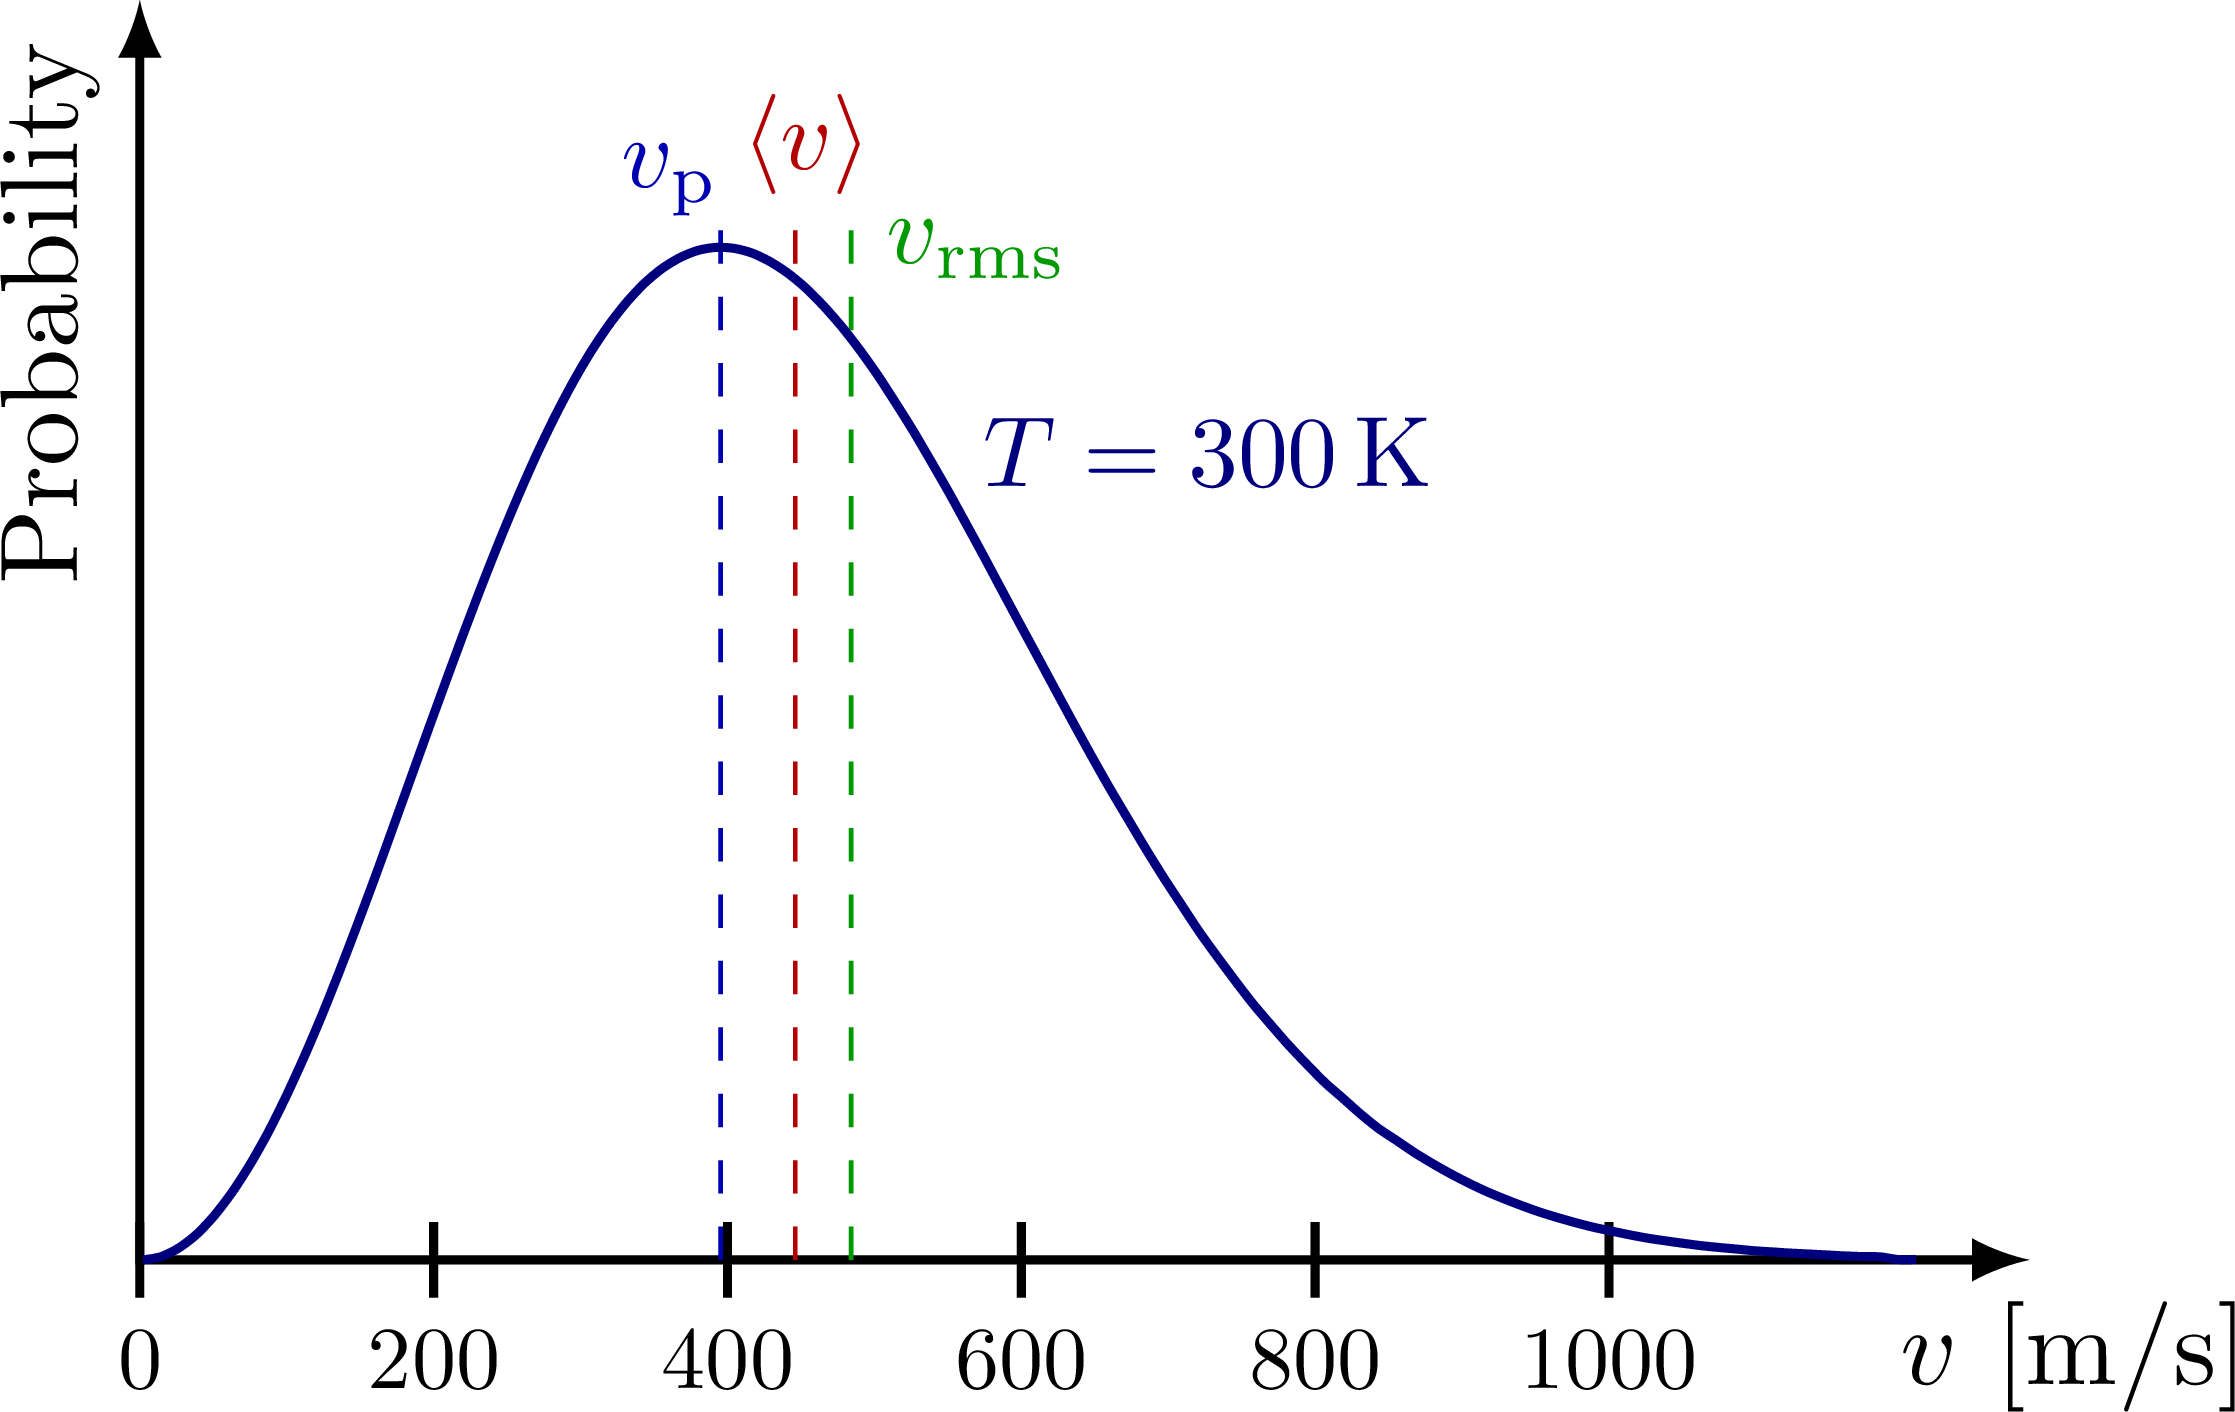
\includegraphics[width=0.9\textwidth]{maxwell-boltzmann-001.png}
	\caption{Annotated speed distribution.}
	\label{fig:maxwell boltzmann}
	\end{subfigure}
	\begin{subfigure}{0.4\textwidth}
		\centering
		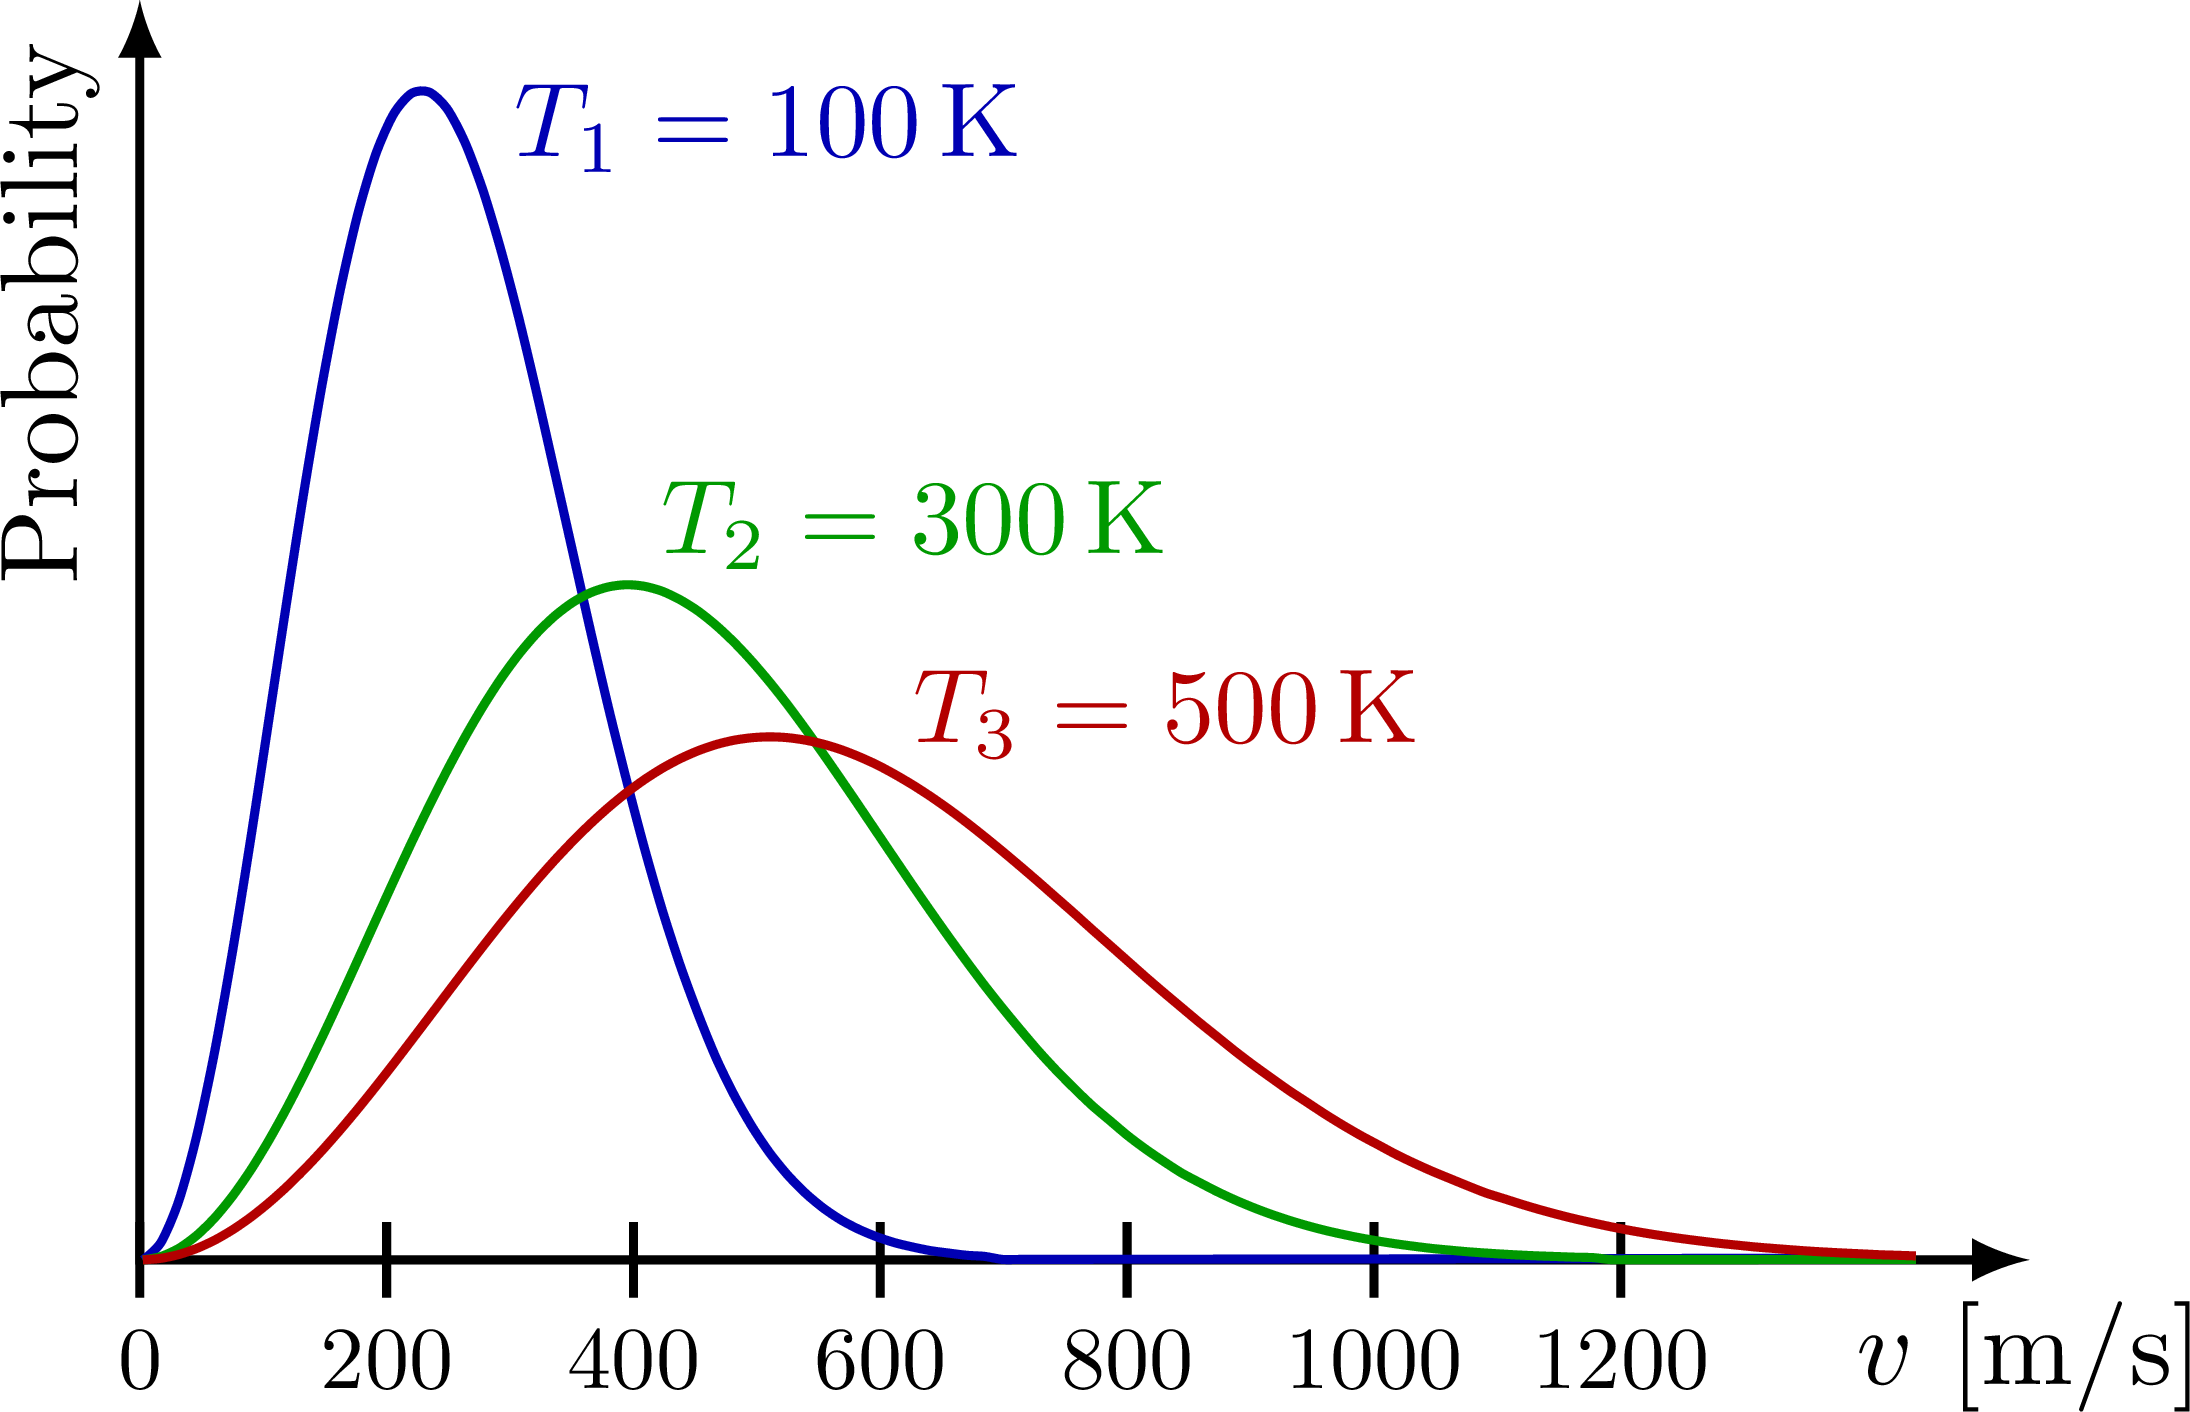
\includegraphics[width=0.9\textwidth]{maxwell-boltzmann-002.png}
		\caption{Speed distribution at other temperatures.}
		\label{fig:maxwell boltzmann 2}
	\end{subfigure}
	\caption{}
\end{figure}
From this we can obtain several different values, which are visualised in figure \ref{fig:maxwell boltzmann},
\begin{align}
	v_p = \sqrt{\frac{2k_BT}{m}} && \left<V\right> = \int_0^{\infty} vp(v) \dd{v} = \sqrt{\frac{8k_BT}{\pi m}} && v_{\text{rms}} = \sqrt{\left<v^2\right>} = \sqrt{\frac{2k_BT}{m}} 
\end{align}
The shape of the distribution changes with temperature, as in figure \ref{fig:maxwell boltzmann 2}.
\section{Equipartition Theorem}
\begin{theorem}
	The average energy due to each degree of freedom that contributes quadratically to the total energy of a classical system in thermal equilibrium at some temperature T is $\frac{1}{2}k_BT$ per particle. 
\end{theorem}
For monatomic moleucles, there are only translational degrees of freedom, i.e., 3 translational degrees of freedom. If we go through with the equipartition theorem, 
\begin{equation}
	\frac{\left<E\right>}{N} = 3 \times \frac{1}{2}k_B T = \frac{3}{2}k_BT
\end{equation}
which agrees with \eqref{eq:energy}.
\subsection{Diatomic Molecules}
\begin{figure}[b]
	\centering
\begin{tikzpicture}[scale=2,z={(0.6,0.4)}]
	\def\z{-.03}
	\def\o{1.03}
	
	\draw[bound] (0,0,0) -- (1,0,0);
	\node at (0.5,0.3,0) {$k$};
	\node at (0.5, -0.3,0) {$\Delta$};
	\fill[atom] (\z,\z,\z) circle (4pt);
	\fill[atom] (\o,\z,\z) circle (4pt);
\end{tikzpicture}
\caption{Diatomic molecule of two molecules seperated by a relative distance $\Delta$, connected by a bond of effective spring constant $k$.}
\label{fig:diatomic}
\end{figure}
If we consider a diatomic molecule composed of identical atoms with some bond between them of an effective spring constant $k$ and relative distance $\Delta$ as in figure \ref{fig:diatomic}, we can seperate the degrees of freedom into three categories and 3 different energies,
\begin{enumerate}
	\item 3 translational degrees of freedom, $E_T = \frac{1}{2}m\left(\Dot{x}^2 + \Dot{y}^2 + \Dot{z}^2\right)$.
	\item 2 rotational degrees of freedom, $E_{\text{rot}} = \frac{1}{2} I_1\Dot{\theta}_1^2 + \frac{1}{2}I_2\Dot{\theta}_2^2$.
	\item 2 vibrational degrees of freedom, $E_{\text{vib}} = \frac{1}{2}m\Dot{\Delta}^2 + \frac{1}{2}k\Delta^2$.
\end{enumerate}
Let us note that the equipartition theorem only applies to classical systems, i.e., when $k_B T >> \Delta E$ where $\Delta E$ is the seperation between discrete energy levels. Furthermore, at lower temperatures, certain degrees of freedom do not contribute to the internal energy. These are,
\begin{align}
	\text{Vibrational} && \text{Rotational} && \text{Translational} \\
	k_BT \sim \Delta E_{\text{vib}} \simeq \hbar \omega && k_BT \sim \Delta E_{\text{rot}} \simeq \frac{\hbar^2}{I} && k_BT \sim \Delta E_{\text{trans}} \simeq \frac{\hbar^2}{mV^{\frac{2}{3}}}
\end{align}
\chapter{Transport Properties of Gasses}

\appendix
\chapter{Definitions}
\textbf{Isothermal Process}:  Happens at constant temperature, $\Delta E = 0$ for an ideal gas.
\\\\
\textbf{Isobaric Process}: Happens at constant pressure.
\\\\
\textbf{Isochoric Process}: Happens at constant volume $\implies \dbar W = 0$.
\\\\
\textbf{Adiabatic Process}: Happens with no heat flow $\implies \dbar Q = 0$.
\\\\
\textbf{Heat Capacity}: Relates heat flow to temperature change $\dbar Q = C \dd{T}$.
\\\\
For an ideal gas at constant volume, the change in energy $\dd{E}$ is always given by,
\begin{equation}
	\dd{E} = C_V \dd{T}
\end{equation}

\end{document}
